% Dissertacao de mestrado
% Andressa Sivolella <asivolella@poli.ufrj.br>
% 2016-02-16

\documentclass[msc,numbers]{coppe}
\usepackage{amsmath,amssymb}
\usepackage{hyperref}
\usepackage[latin1]{inputenc}
\usepackage[brazil]{babel}
\usepackage{graphicx}% Include figure files
\usepackage{multirow}
\usepackage{indentfirst}
\usepackage{subfigure}
\usepackage{url}
\usepackage{float}
\usepackage{textcomp}
\usepackage{tikz}
\usetikzlibrary{shapes,arrows}

\makelosymbols
\makeloabbreviations

\begin{document}
  \title{
    Intelig�ncia Computacional na Avalia��o de C�digos em um Sistema Complexo de Detec��o com Desenvolvimento Colaborativo
  }
  \foreigntitle{
    Computational Intelligence in Source Code Assertion in a Complex System in a Collaborative Development Enviroment
  }
  \author{Andressa A.}{Sivolella Gomes}
  \advisor{Prof.}{Jos�}{Manoel de Seixas}{D.Sc.}

  \examiner{Prof.}{Alu�zio Fausto Ribeiro Ara�jo}{D.Sc.}
  \examiner{Prof.}{Afonso de Bediaga e Hickman}{D.Sc.}
  \examiner{Pesquisadora}{Carmen L�cia Lodi Maidantchik}{D.Sc.}
  \department{PEE}
  \date{03}{2016}

  \keyword{Minera��o de c�digos}
  \keyword{M�todos ensemble com �rvores}
  \keyword{Plataforma colaborativa}

  \maketitle

  \frontmatter
  \dedication{A todo mundo, geralz�o.}

  \chapter*{Agradecimentos}

  Gostaria de agradecer a todos.

  \begin{abstract}

  Apresenta-se, nesta tese, ...

  \end{abstract}

  \begin{foreignabstract}

  In this work, we present ...

  \end{foreignabstract}

  \tableofcontents
  \listoffigures
  \listoftables
  \printlosymbols
  \printloabbreviations

  \mainmatter

  \chapter{Introdu��o}
    No desenvolvimento de projetos de software, quanto mais cedo uma falha em c�digo � identificada, menos custosa � a sua manuten��o. Uma das maneiras de garantir qualidade est� na utiliza��o de analisadores est�ticos: tal ferramenta gera alertas sem a necessidade de execu��o do c�digo que est� sendo desenvolvido. Tais alertas indicam linhas em que possivelmente o c�digo ir� falhar quando em execu��o. Mas, com o passar do tempo, um inconveniente do analisador est�tico foi empiricamente identificado: percebeu-se que a maior parte dos alertas gerados n�o indica necessariamente falha em tempo de execu��o e em contra partida, algumas falhas nem sequer s�o identificadas pelos alertas do analisador est�tico.
    
    Neste contexto, uma aplica��o que surge para auxiliar a �rea de engenharia de software na oferta de qualidade em desenvolvimento de codigo fonte � a �rea de intelig�ncia computacional aplicada em c�digos. As motiva��es s�o diversas: v�o desde minera��o em repositorios de versionamento para identifica��o do que determinado projeto faz sem nem ao menos execut�-lo, at� a identifica��o de trechos de c�digos em grandes projetos que s�o muito similares (ou at� mesmo iguais) e dificultam a sua manuten��o.

    Este projeto �, portanto, interdisciplinar e busca aplicar t�cnicas de intelig�ncia computacional durante o desenvolvimento de software.
    \section{Motiva��o}
    O CERN (Organiza��o Europ�ia de Pesquisa Nuclear) possui em opera��o o LHC (\emph{Large Hadron Colider}), que � o maior colisor de part�culas j� constru�do na hist�ria. Ao longo do LHC foram constru�dos experimentos, que s�o pontos de observa��o onde as part�culas aceleradas em dire��es opostas se colidem.
    O ATLAS � o experimento o qual este projeto est� inserido. Sua colabora��o � composta por milhares de pessoas e dezenas de pa�ses membros. O calor�metro de telhas (TileCal) comp�e o sistema de calorimetria do ATLAS juntamente com o calor�metro de arg�nio l�quido, e tem como objetivo medir a energia das part�culas resultantes de colis�es.
    Um dos objetivos da colabora��o do TileCal � assegurar a qualidade de dados de calibra��o para garantir a sua opera��o. Uma caracter�stica marcante de projetos no CERN � a alta rotatividade de pesquisadores dentro do experimento. Um novo entrante no projeto ou a simples troca de fun��es exige um tempo de treinamento. Muitas s�o as tarefas que precisam
    ser realizadas pela equipe que analisa os resultados gerados, a fim de garantir a qualidade de dados do TileCal. A maior parte dessas tarefas � realizada com o aux�lio de sistemas computacionais desenvolvidos ao longo da colabora��o de diferentes institutos. Para facilitar a integra��o de tais ferramentas, a Plataforma web Tile-in-ONE foi desenvolvida e uma de suas principais caracter�sticas � fornecer um ambiente via web para o desenvolvimento de an�lises f�sicas atrav�s da implementa��o de c�digos fonte.
    O Tile-in-ONE foi projetado para executar os c�digos desenvolvidos e compartilhados pela colabora��o em um conjunto de m�quinas separadas do servidor para evitar sobrecarga de processamento ou acesso a dados. Atualmente a plataforma encontra-se em produ��o.
    Se um c�digo fonte � submetido com falhas, consome-se tempo e recursos computacionais ao enviar o c�digo para m�quinas diferentes do servidor. Neste contexto, surge uma quest�o: seria poss�vel identificar c�digos fonte com potencial de falha sem necessariamente execut�-los? O projeto aqui desenvolvido busca responder tal pergunta.
    \section{Objetivos}
    \label{objetivos}
    Como dito anteriormente, este projeto tem como objetivo principal identificar c�digos fonte com falhas, desenvolvidos em um ambiente web colaborativo, antes de sua execu��o, evitando que recursos computacionais sejam utilizados sem necessidade.
    Algor�tmos de aprendizado de m�quina ser�o verificados como uma maneira de abordar o objetivo principal deste projeto. Esta avalia��o pode se dar atrav�s de medidas e ferramentas frequentemente utilizadas na �rea de intelig�ncia computacional (F1-score e matrizes de confus�o, principalmente).
    A investiga��o de aplica��o de intelig�ncia computacional na �rea de F�sica de Altas Energias para este fim e a aplica��o de ferramentas que garantem a qualidade de c�digos desenvolvidos tamb�m � um dos objetivos deste projeto.
    \section{Organiza��o do documento}
    No Cap�tulo~\ref{cern} o ambinete do CERN, o colisor de part�culas LHC e o experimento ATLAS s�o apresentados, com �nfase no Calor�metro de Telhas (TileCal) bem como suas an�lises e os diferentes grupos que comp�em a colabora��o TileCal.

    O Cap�tulo~\ref{tio} descreve a Plataforma web Tile-in-ONE projetada e desenvolvida, desde o fluxo de dados projetado, at� mesmo a infraestrutura implantada. Ao ser colocado em produ��o uma nova necessidade surge e tal necessidade tamb�m � descrita neste cap�tulo.

    Uma investiga��o na literatura sobre a aplica��o de minera��o de c�digos para a identifica��o de falhas em c�digos sem a sua execu��o � abordada no cap�tulo~\ref{code_mining}, principalmente no ambiente de F�sica de Altas Energias, e consequentemente, no CERN. Neste cap�tulo tamb�m s�o abordados os atributos comumente utilizados na aplica��o de minera��o em c�digos. Os algoritmos que foram testados como uma poss�vel abordagem o finalizam.

    O Cap�tulo~\ref{results} descreve quais c�digos fonte comp�em o conjunto de dados que foi utilizado para o treinamento dos algoritmos descritos no cap�tulo anterior. Faz-se um estudo tamb�m da necessidade em se utilizar todos os atributos citados pela literatura. E por fim, o desempenho dos classificadores gerados s�o discutidos.

    O Cap�tulo~\ref{conclusoes} finaliza este documento avaliando se os objetivos descritos na se��o~\ref{objetivos} foram contemplados e levanta ainda algumas poss�veis an�lises que podem ser abordadas no futuro.
  \chapter{A Colabora��o ATLAS do CERN}
    \section{CERN e LHC}
    Fundado em 1954, o CERN (em franc�s \emph{Centre Europ�en pour la Recherch� Nucl�aire}~\cite{CERN}) � o maior centro de pesquisa na �rea de f�sica de part�culas de altas energias no mundo. Atualmente, conta com a participa��o de 38 pa�ses membros e outros pa�ses colaboradores, entre eles o Brasil.

    O LHC (em ingl�s \emph{Large Hadron Collider}~\cite{LHC}) � o maior colisor de part�culas j� constru�do e encontra-se atualmente em opera��o no CERN. Instalado a 175 metros abaixo do solo, consiste em um grande t�nel em formato anelar, com 27 km de per�metro.
    \begin{figure}[htbp]
      \centering
        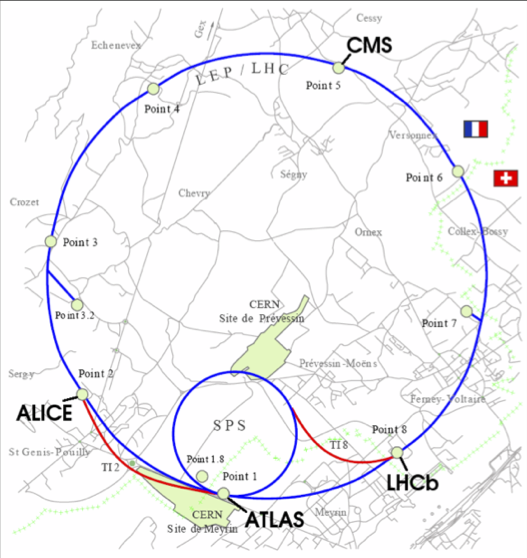
\includegraphics[width=9.0cm]{images/lhc-upper.png}
        \caption{Representa��o a�rea do LHC e seus detectores no CERN. Extra�do de~\cite{CDS}.}
      \label{LHC}
    \end{figure}
    Quando part�culas s�o eletricamente carregadas e submetidas a pulsos eletromagn�ticos no interior de tubos tem-se o processo de acelera��o de part�culas. Neste processo, as part�culas adquirem acelera��o ao serem envolvidas a campos eletromagn�ticos variantes~\cite{GRIFFITHS}. Em aceleradores circulares, part�culas s�o injetadas e circulam no anel at� atingirem a energia desejada. Diversos experimentos podem ser realizados em determinados pontos de colis�o ao longo da circunfer�ncia. O per�metro do acelerador circular � diretamente proporcional a energia necess�ria na colis�o. Ao atingir a energia desejada, os feixes de part�culas aceleradas em sentidos opostos colidem e, nesse caso, detectores em formato cil�ndrico s�o os mais utilizados. Cada colis�o gera informa��es que devem ser analisadas por especialistas, com objetivos distintos, tais como: identifica��o de sub-part�culas, observa��o de fen�menos e a comprova��o ou a elimina��o de teorias f�sicas. Nos pontos de colis�o, detectores s�o montados para observa��o e coleta de dados. Existem, por exemplo, detectores de calorimetria, para identificar a energia depositada pelas part�culas colisionadas; detectores de tra�os, para observar trajet�rias ap�s colis�es; e detectores de m�ons, respons�veis por absorver tais part�culas.


    A figura~\ref{LHC} ilustra uma representa��o a�rea do LHC. Existem quatro detectores de part�culas instalados em pontos de colis�o ao longo da extens�o do LHC, altamente especializados: ALICE~\cite{ALICE}, ATLAS~\cite{ATLAS}, CMS~\cite{CMS} e LHCb~\cite{SZUMLAK2010}.
    Os detectores ilustrados permitem obter informa��es detalhadas sobre a trajet�ria das part�culas resultantes das colis�es ocorridas e caracter�sticas energ�ticas, sendo poss�vel identificar part�culas. O ATLAS � o maior dos detectores do LHC.

    \section{Experimento ATLAS}
    O ATLAS (em ingl�s \emph{A Toroidal LHC AparatuS})~\cite{ATLAS} � um detector em formato cil�ndrico. O detector pesa aproximadamente 7.000 toneladas, com 44 metros de comprimento por 24 metros de altura. A figura~\ref{ATLAS} ilustra os diversos subsistemas que comp�em o detector ATLAS.

    Cada subsistema apresenta uma caracter�stica espec�fica de acordo com suas funcionalidades. S�o eles, da parte interna para a externa:
    \begin{itemize}
      \item{Detector Interno (ID)}, respons�vel por registrar as trajet�rias
        das part�culas resultantes da colis�o, bem como o momento e o sinal
        da carga, se for o caso;
      \item{Sistema de Calorimetria}, composto pelos calor�metros
        eletromagn�tico (LAr) e hadr�nico de telhas (TileCal). Os calor�metros citados s�o respons�veis por medirem a energia das part�culas resultantes;
      \item{Sistema Magn�tico}, respons�vel por desviar part�culas carregadas
        para medir o momento;
      \item{o Espectr�metro de M�ons}, respons�vel por medir a trajet�ria de
        uma determinada part�cula denominada M�on.
    \end{itemize}

    \begin{figure}[htbp]
      \centering
        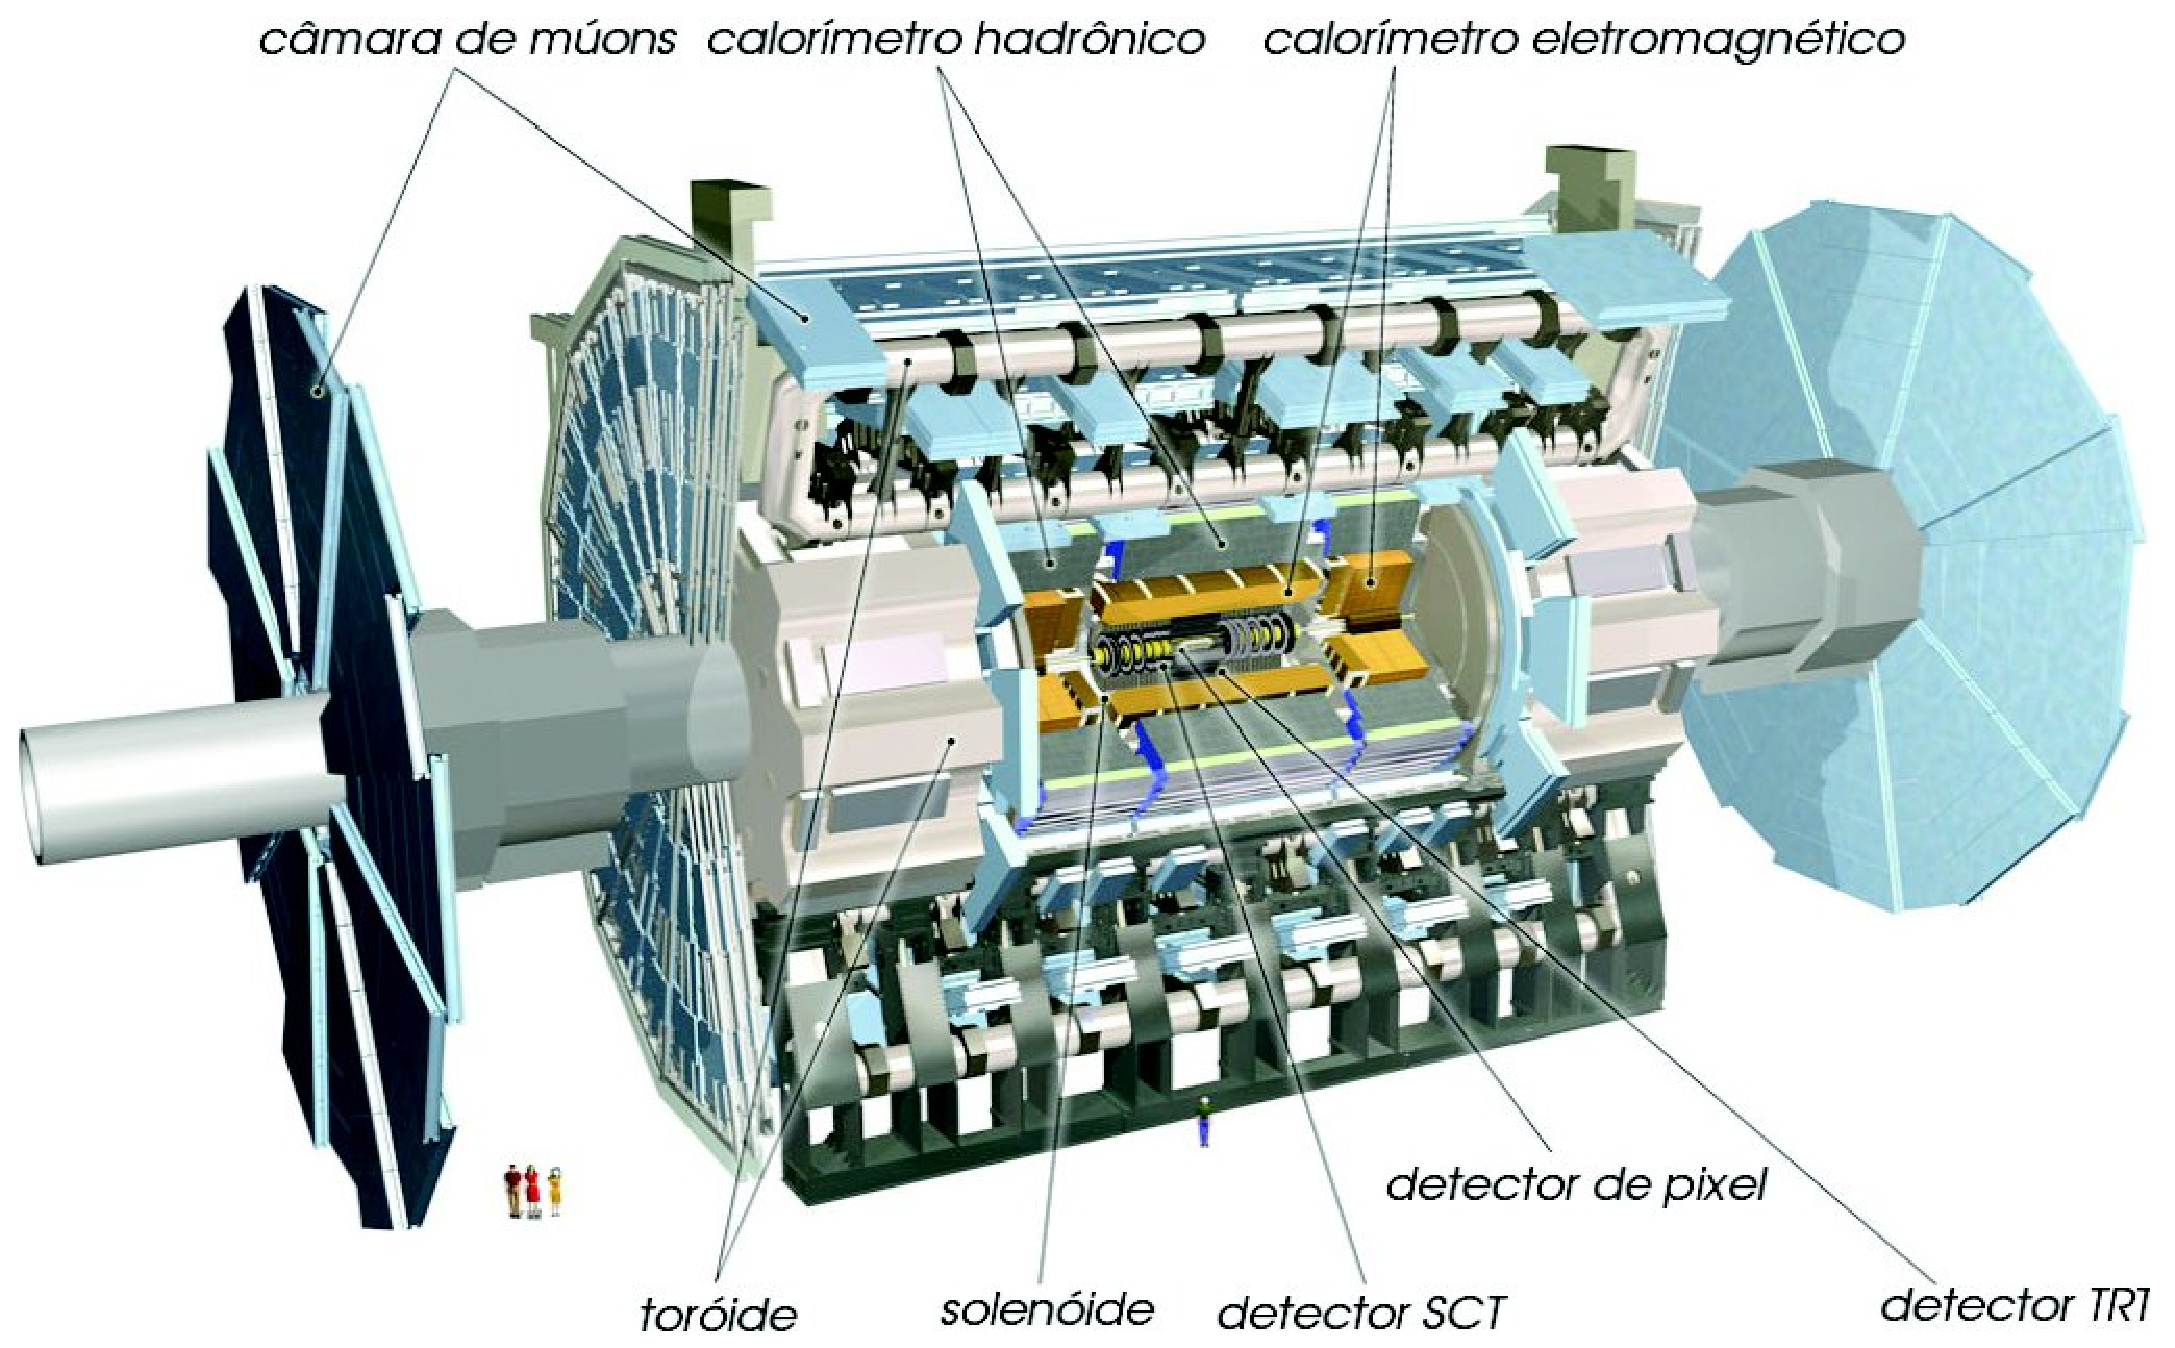
\includegraphics[width=12.0cm,height=8cm]{images/ATLAS_esquema.eps}
        \caption{Esquema do detector ATLAS. Adaptado de~\cite{ATLASPHOTOS}}
      \label{ATLAS}
    \end{figure}
    O sistema de calorimetria do LHC foi projetado para absorver a energia das part�culas que cruzam o detector, sendo o calor�metro hadr�nico de telhas (em ingl�s \emph{Tile Calorimeter} ou TileCal) � o foco deste mestrado.

    \section{Calor�metro Hadr�nico de Telhas (TileCal)}
    O TileCal~\cite{TDR_Tile} � composto por tr�s barris: um central (que se divide em duas parti��es: LBA e LBC) e dois estendidos (cada um correspondendo a mais duas parti��es, EBA e EBC, respectivamente), como ilustrado na figura~\ref{TILECAL_BARRELS}. Cada parti��o � igualmente dividida em 64 partes (m�dulos). Os m�dulos do TileCal s�o compostos de ferro como mediadores passivos e telhas cintilantes como material ativo. A estrutura absorvedora � coberta de placas de a�o de v�rias dimens�es, conectadas a uma estrutura maci�a de suporte. A principal inova��o deste detector � a posi��o perpendicular das telhas em rela��o aos feixes do LHC.

    \begin{figure}[htbp]
      \centering
        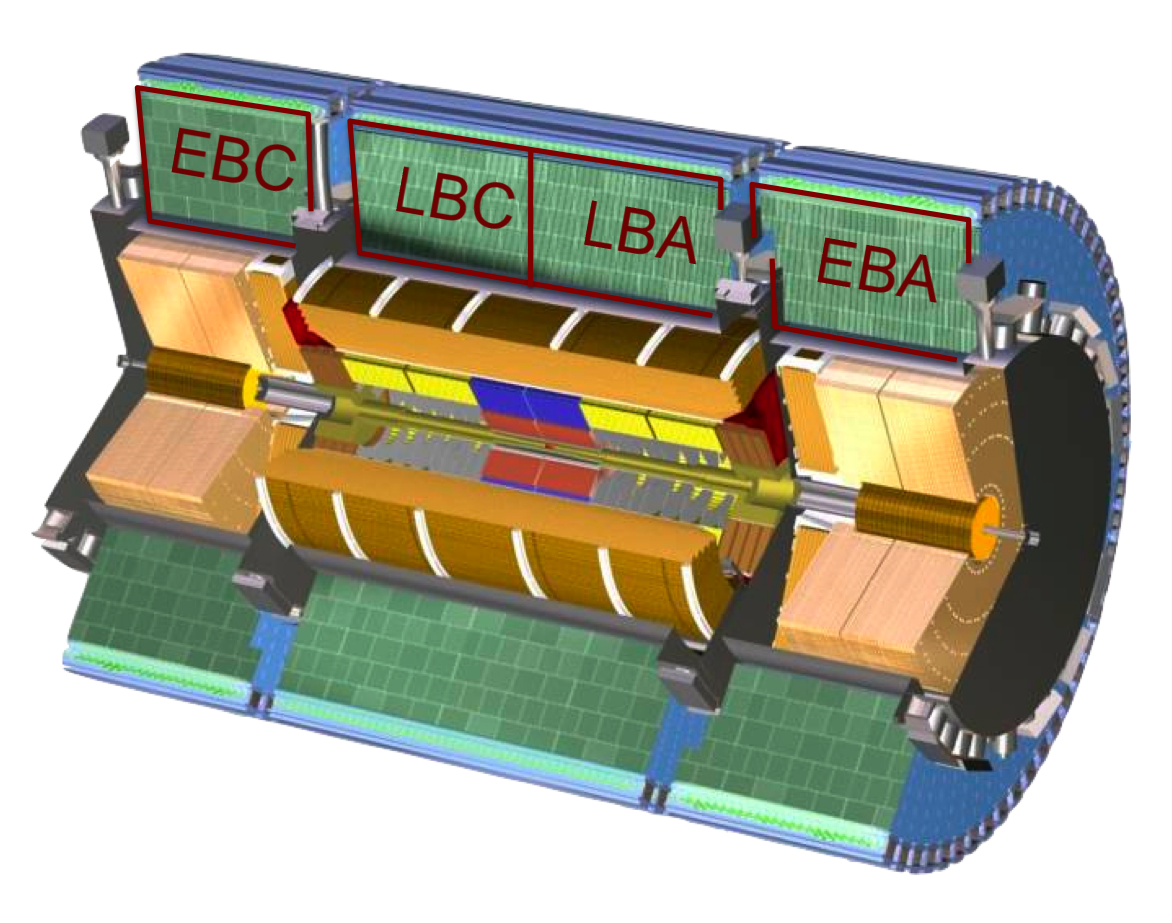
\includegraphics[width=10.0cm]{images/TileCal_barrels.png}
        \caption{Calor�metro de Telhas do ATLAS (com suas 4 parti��es na cor
          verde) envolvendo o calor�metro de arg�nio l�quido. O Sistema Magn�tico
        e a C�mara de M�ons n�o est�o ilustrados nesta figura. Adaptado de~\cite{ATLAS}.}
      \label{TILECAL_BARRELS}
    \end{figure}

    A passagem de part�culas ionizadas pelo TileCal produz luz no espectro. Sua
    intensidade � proporcional � energia depositada pela part�cula. A luz produzida
    se propaga atrav�s das telhas para suas bordas onde � absorvida por fibras
    �ticas e deslocada, por reflex�o interna total, at� os canais de leitura
    eletr�nica ou fotomultiplicadores (em ingl�s \emph{PhotoMulTipliers Tubes} ou
    PMTs), onde � convertido em um sinal de corrente. Um PMT pode ser idealizado
    como um pulso de corrente. A figura~\ref{TILECAL_PMT-FIG} ilustra a estrutura
    de absor��o e amostragem do TileCal sendo poss�vel identificar tubos
    fotomultiplicadores.

    \begin{figure}[htbp]
      \centering
        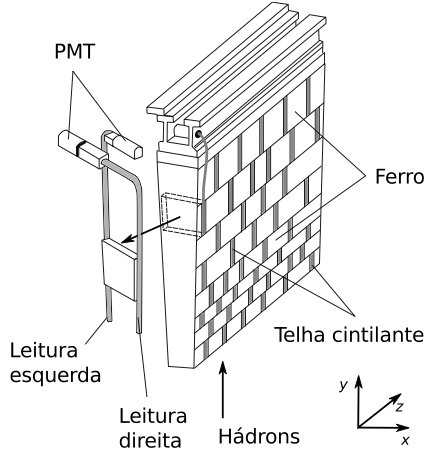
\includegraphics[width=7.0cm]{images/tilecal_pmt.png}
        \caption{Estrutura de absor��o e amostragem do TileCal. Extra�do de~\cite{TDR_Tile}}
      \label{TILECAL_PMT-FIG}
    \end{figure}

    Os m�dulos do barril central do detector comportam 45 canais cada, enquanto os m�dulos dos barris estendidos comportam 32 canais. Radialmente, cada m�dulo do TileCal ainda � segmentado em tr�s camadas (A, BC e D), conhecidas como c�lulas. Estas s�o formadas pelo agrupamento de fibras at� cada PMT. Um esbo�o da geometria das c�lulas � apresentado na figura~\ref{TILECAL_CELLS-FIG}. Cada m�dulo cont�m 11 linhas transversas de telhas.

    \begin{figure}[htbp]
      \centering
        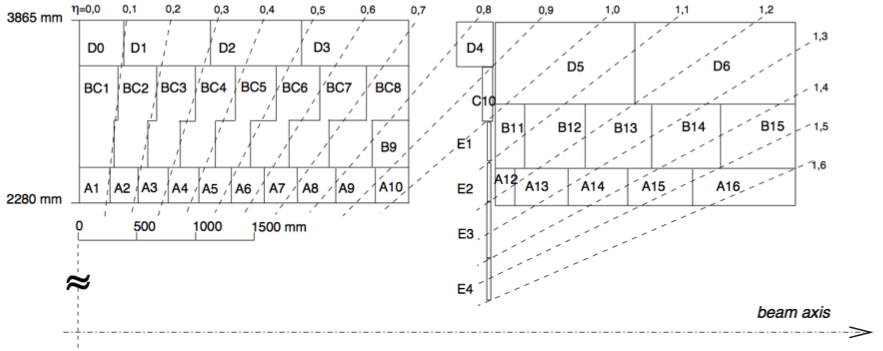
\includegraphics[width=12.0cm]{images/tilecal_cells.png}
        \caption{Esbo�o das c�lulas do TileCal. Extra�do de~\cite{ATLAS}.}
      \label{TILECAL_CELLS-FIG}
    \end{figure}

        \subsection{An�lise \emph{Online} e \emph{Offline}}
        Existem dois tipos de an�lises, comuns a todos os experimentos do LHC. O experimento ATLAS, sozinho, gera um volume de dados na ordem de 3,2 PetaBytes ao ano~\cite{ATLAS_FACTS}, que precisam ser processados e analisados. Nesse caso, � impratic�vel armazenar os dados adquiridos pelo experimento em sua totalidade para posterior an�lise. Por esse motivo, an�lises referentes a atividades anteriores ao armazenamento em m�dia permanente s�o definidas como \emph{online}. J� as an�lises que ocorrem a partir do acesso de informa��es em bases de dados s�o definidas como sendo \emph{offline}.

        As solu��es abordadas neste mestrado est�o contextualizadas no processo de an�lise \emph{offline} do TileCal.

        As an�lises \emph{online} e \emph{offline} ser�o descritas detalhadamente na se��o~\ref{tio}.

        \subsection{A colabora��o TileCal}
        O TileCal � composto ainda por diferentes grupos, respons�veis por atividades espec�ficas no experimento. Cada grupo desempenha uma etapa no processo de trabalho do calor�metro. S�o eles:

        \begin{description}
          \item[DAQ (do ingl�s, \emph{Data Acquisition} ou aquisi��o de dados)]
            respons�vel pela aquisi��o dos sinais resultantes das intera��es
            f�sicas no detector;
          \item[DCS (do ingl�s, \emph{Detector Control System}, ou sistema de
            controle do detector)] respons�vel pela manuten��o das fontes de alta e
            baixa tens�o do TileCal, placas m�e e sistema de refrigera��o;
          \item[DQ (do ingl�s, \emph{Data Quality}, ou qualidade de dados)]
            respons�vel por avaliar o funcionamento do detector garantindo
            confiabilidade nos dados adquiridos que ser�o analisados;
          \item[Calibra��o (do ingl�s, \emph{Calibration})] respons�vel pela
            calibra��o das c�lulas do calor�metro e valida��o da escala
            eletromagn�tica, a fim de corrigir desvios que ocorrem ao longo do
            tempo devido a desgastes ocorridos
            pela exposi��o do detector a altos n�veis de radia��o;
          \item[Computa��o e Software] respons�vel por realizar a organiza��o e
            desenvolvimento da simula��o, reconstru��o, digitaliza��o e
            desenvolvimento de filtros de alto n�vel;
          \item[Dados e Processamento (do ingl�s, \emph{Data and Processing})]
            respons�vel por coletar informa��es dos grupos de qualidade de dados e
            calibra��o a fim de decidir que altera��es nos dados de condi��es ser�o
            realizadas. Respons�vel tamb�m por analisar os dados f�sicos.
        \end{description}

        Existem, portanto, seis grupos no TileCal onde o compartilhamento de informa��es entre eles faz-se necess�rio: se um PMT n�o est� sendo corretamente alimentado, a qualidade dos dados adquiridos pode ficar comprometida. Tal situa��o exige o compartilhamento de informa��es do grupo e DQ, por exemplo.
  \chapter{Plataforma web Tile-in-ONE}
\label{tio}
Diversos sistemas foram desenvolvidos ao longo das diferentes fases do experimento, cada um com um prop�sito espec�fico~\cite{CHEP2010-DASHBOARD}. A an�lise \emph{online} tem in�cio com a aquisi��o e decis�o acerca do armazenamento dos dados adquiridos, que � responsabilidade do grupo TDAQ (do ingl�s, \emph{Trigger and Data Acquisition})~\cite{jenni2003atlas}. A reconstru��o dos dados pelo software para an�lise \emph{offline} ATHENA~\cite{ATHENA} marca o in�cio da an�lise \emph{offline}. Em seguida, o DQMF (do ingl�s, \emph{Data Quality Monitoring Framework})~\cite{DQMF} � aplicado e gera automaticamente estados para os PMTs, indicando a qualidade do tubo fotomultiplicador e reduzindo a quantidade de canais que precisam ser analisados. Nesta etapa, gr�ficos s�o gerados para auxiliar o grupo de qualidade de dados do TileCal em sua an�lise \emph{offline}. Um sistema web foi desenvolvido para integrar os resultados gr�ficos gerados durante a etapa de reconstru��o, guiando o grupo de qualidade de dados em suas an�lises. A figura~\ref{dashboard} ilustra sistemas integrados por uma �nica interface web: a figura~\ref{fig:dashboard_1} corresponde � lista de dados reconstru�dos e quais gr�ficos j� est�o dispon�veis para a colabora��o, indicando que a atua��o do ATHENA foi conclu�da; a figura~\ref{fig:dashboard_2} exibe informa��o detalhada sobre um determinado m�dulo, acessado pela interface ilustrada anteriormente. Atrav�s deste sistema web � poss�vel inserir coment�rios relacionados � performance do detector; e a figura~\ref{fig:dashboard_3} ilustra alguns gr�ficos gerados durante a etapa de reconstru��o dos dados.
\begin{figure}[!ht]
  \centering
  \subfigure[Lista dos dados adquiridos.]{
    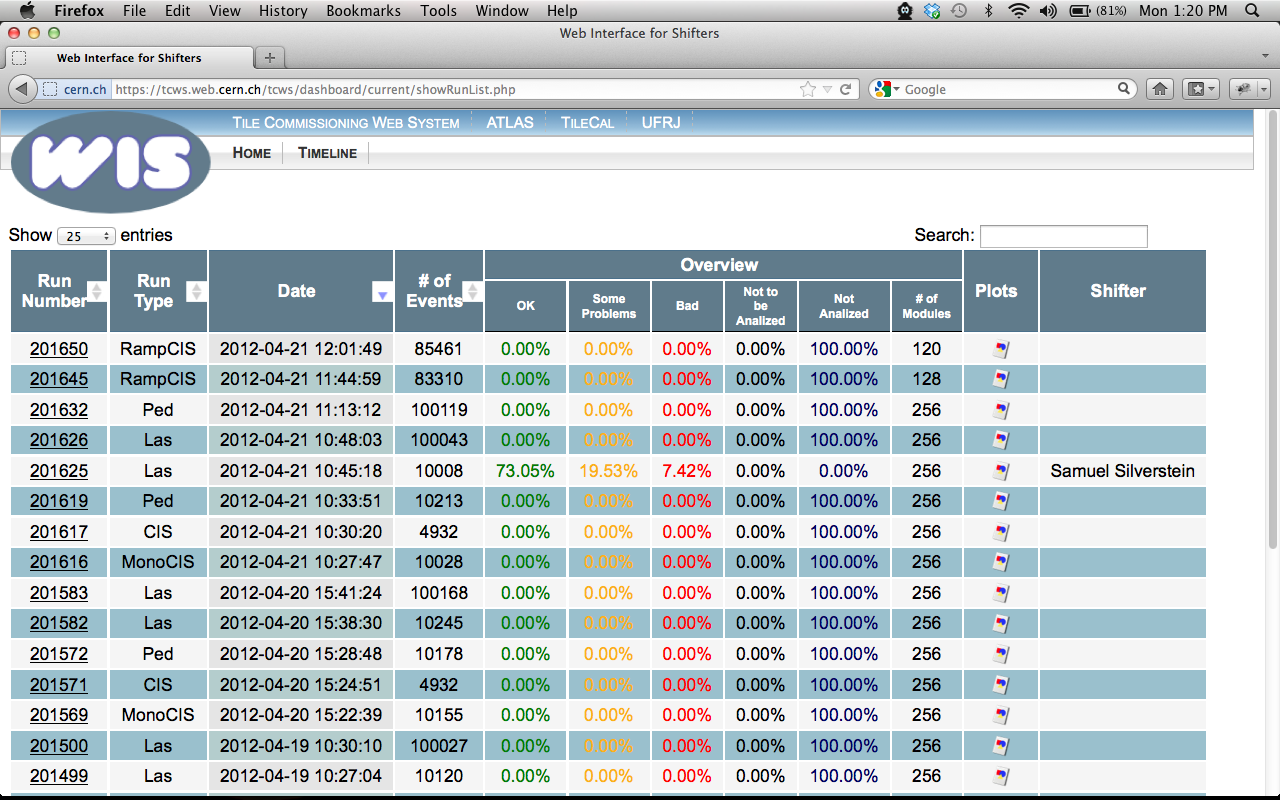
\includegraphics[width=10cm]{images/screen-capture-5.png}
    \label{fig:dashboard_1}
  }
  \mbox{
    \subfigure[Estados gerados automaticamente pelo DQMF e acesso a informa��es detalhadas.]{
      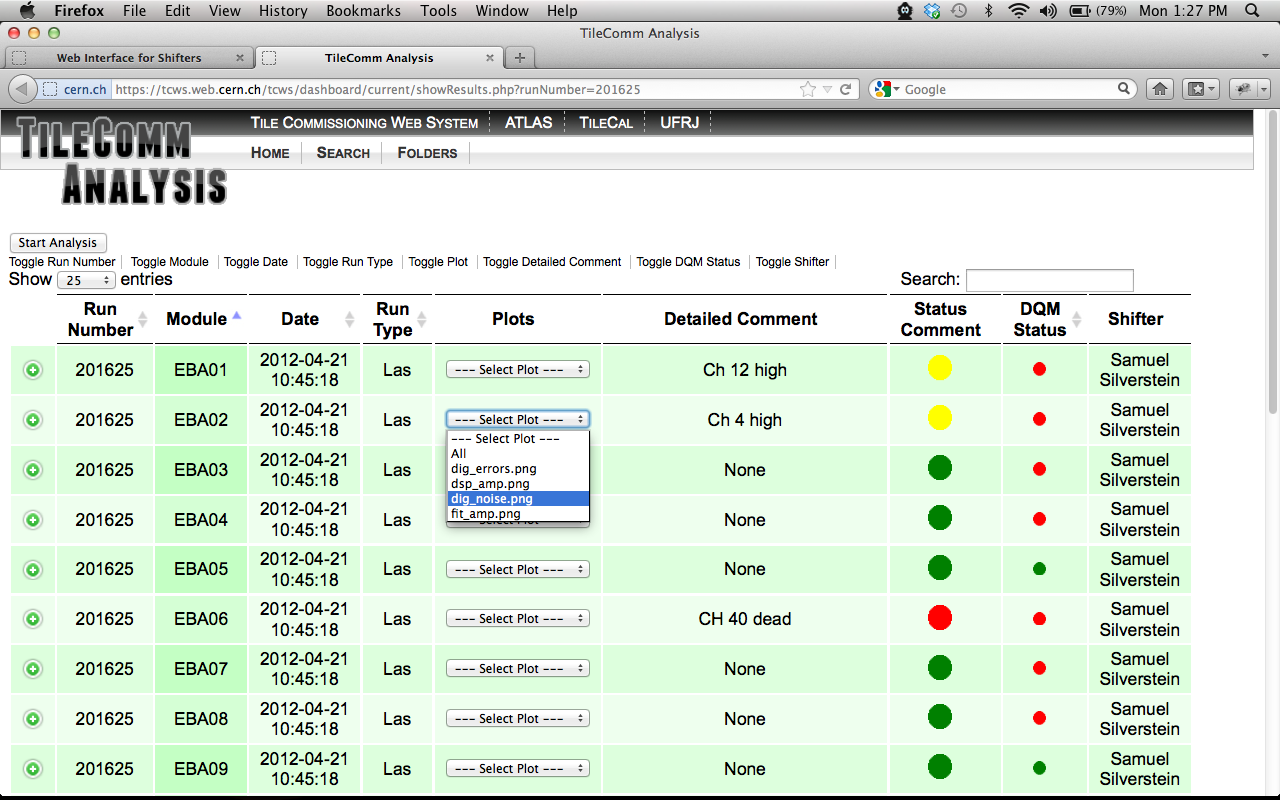
\includegraphics[width=6.5cm]{images/screen-capture-6.png}
      \label{fig:dashboard_2}
    }
    \subfigure[Gr�ficos gerados para um determinado m�dulo.]{
      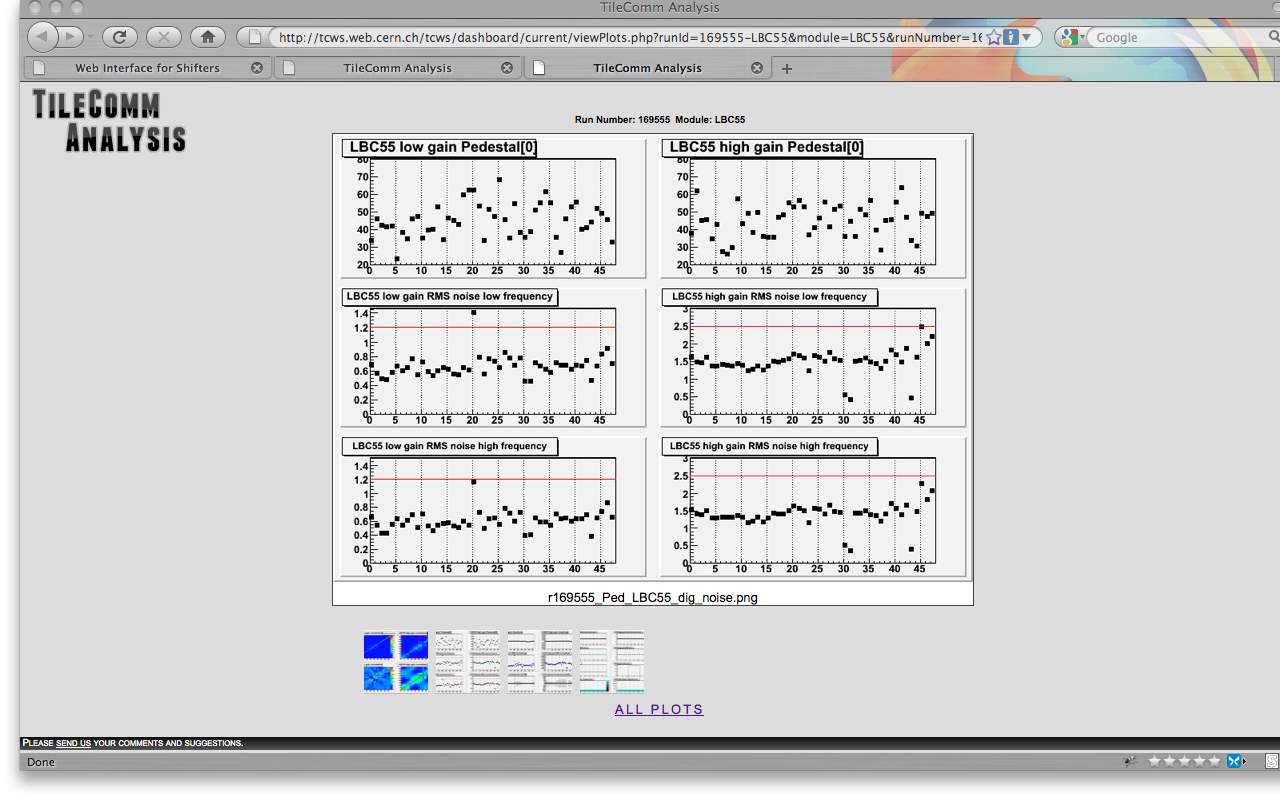
\includegraphics[width=6.5cm]{images/screen-capture-7.png}
      \label{fig:dashboard_3}
    }
  }
  \caption{\emph{Dashboard Web System}, desenvolvido em 2010 para integrar as os dados adquiridos e as an�lises do grupo de QD do TileCal. Mais detalhes em~\cite{CHEP2010-DASHBOARD}.}
  \label{dashboard}
\end{figure}

Para uma refer�ncia hist�rica, a lista de canais definidos como defeituosos pela colabora��o (\emph{Bad Channels List}) � armazenada no banco de dados de condicionamento, comum a todos os experimentos que comp�em o LHC, o COOL DB~\cite{COOL_DB}. Os sistemas MCWS (do ingl�s, \emph{Monitoring \& Calibration Web System})~\cite{MCWS-CHEP-2012} e DCS (do ingl�s, \emph{Detector Control System})~\cite{DCS-CHEP-2009} ap�iam o grupo de qualidade de dados na an�lise dos quase 10.000 PMTs do calor�metro de telhas. O MCWS foi desenvolvido para exibir a lista de canais defeituosos de maneira gr�fica e permite que coment�rios sobre o estado do detector sejam compartilhados. O sistema web DCS foi desenvolvido para monitorar as fontes de alta tens�o que alimentam os PMTs.

� evidente que o cen�rio descrito � composto por diversas ferramentas (web) para apoiar em diferentes aspectos as an�lises e opera��o de forma mais eficiente do TileCal. Tais sistemas foram desenvolvidos em diferentes fases do detector, envolvendo colaboradores diversos, que n�o necessariamente ainda encontram-se envolvidos em atividades da colabora��o. Al�m disso, a manuten��o de tais ferramentas n�o � garantida pelos mesmos colaboradores contribuintes. Para a colabora��o, seria mais f�cil reunir as ferramentas existentes em uma �nica interface, que utilizasse preferencialmente a mesma tecnologia, permitindo inclusive, centraliza��o de c�digos fonte. Tais requisitos foram abordados com o projeto e desenvolvimento da Plataforma web Tile-in-ONE, durante o desenvolvimento desta disserta��o.

    \section{Fluxo de dados}

    A Plataforma Tile-in-ONE foi projetada para integrar as diferentes an�lises realizadas pela colabora��o TileCal. Ao fornecer uma estrutura onde os colaboradores podem desenvolver c�digos fonte diretamente atrav�s da web, ela re�ne diferentes resultados de an�lises em um �nico lugar. Inicialmente, a escolha pela linguagem de programa��o Python~\cite{PYTHON} � estimulada para novos desenvolvimentos, o que torna a manuten��o da plataforma mais f�cil. Al�m disso, existe o incentivo natural para reutiliza��o de c�digos, uma vez que os desenvolvimentos encontram-se dispon�veis e centralizados para toda colabora��o. Outra funcionalidade oferecida pela plataforma � o encapsulamento em pacotes de configura��es para acessar bases de dados importantes para as an�lises. Isso permite que colaboradores novos n�o percam tempo aprendendo a acessar a informa��o, mas foquem na an�lise propriamente dita.

    A figura~\ref{fig:dataflow} ilustra o fluxo de dados do Tile-in-ONE. A plataforma oferece a funcionalidade de desenvolvimento de c�digos pela qual os colaboradores podem escrever seus pr�prios programas. Tamb�m � permitida a edi��o de c�digos salvos ou escritos por outros usu�rios. Uma vez que o desenvolvimento do c�digo � conclu�do, o desenvolvedor pode submeter seu c�digo que ser� manipulado no lado do servidor. Este, por sua vez, ir� direcionar o c�digo em quest�o para uma outra m�quina (nesse contexto, m�quinas \emph{slaves}), dependendo dos dados identificados pela plataforma que o c�digo fonte a ser executado deseja acessar. Cada m�quina \emph{slave} est� configurada para acessar um determinado reposit�rio de dados utilizado para as an�lises da colabora��o. Isso permite que os desenvolvedores se abstraiam de configura��es de acesso a tais reposit�rios. A motiva��o para efetuar a execu��o do c�digo fonte em outra m�quina que n�o no servidor � evitar que ocorra sobrecarga no servidor principal e o mais importante: caso o c�digo fonte falhe durante a execu��o, o servidor onde a plataforma est� hospedado n�o fica comprometido. A figura~\ref{fig:dataflow} ilustra ainda, em vermelho, onde esta tese de mestrado ir� atuar. O objetivo � criar uma etapa antes da submiss�o de novos c�digos para m�quinas \emph{slave}, atuando, desta forma, como uma camada de seguran�a cujo intuito � prever quais c�digos v�o falhar sem a necessidade de execut�-los. Esta camada consiste em um novo desenvolvimento e portanto, no momento, qualquer c�digo pode ser submetido para ser executado na m�quina \emph{slave}.

    Uma vez que o servidor web escolhe uma m�quina \emph{slave} esta tenta executar o c�digo fonte submetido e retorna para o servidor web, de maneira estruturada, o que ocorreu durante a execu��o. Neste momento, o desenvolvedor do c�digo fonte pode utilizar objetos gr�ficos tamb�m fornecidos pela plataforma para exibir os resultados recuperados atrav�s de seus c�digos fonte. Enfim, o c�digo fonte, a resposta obtida com a execu��o na m�quina \emph{slave} e os objetos gr�ficos s�o encapsulados em \emph{Plugins} e disponibilizados em \emph{Dashboards} para toda colabora��o.

    A figura~\ref{fig:infrastructure} ilustra a infraestrutura atual da plataforma web Tile-in-ONE. Destaca-se em vermelho onde este mestrado pretende atuar.

    \begin{figure}[H]
      \centering
      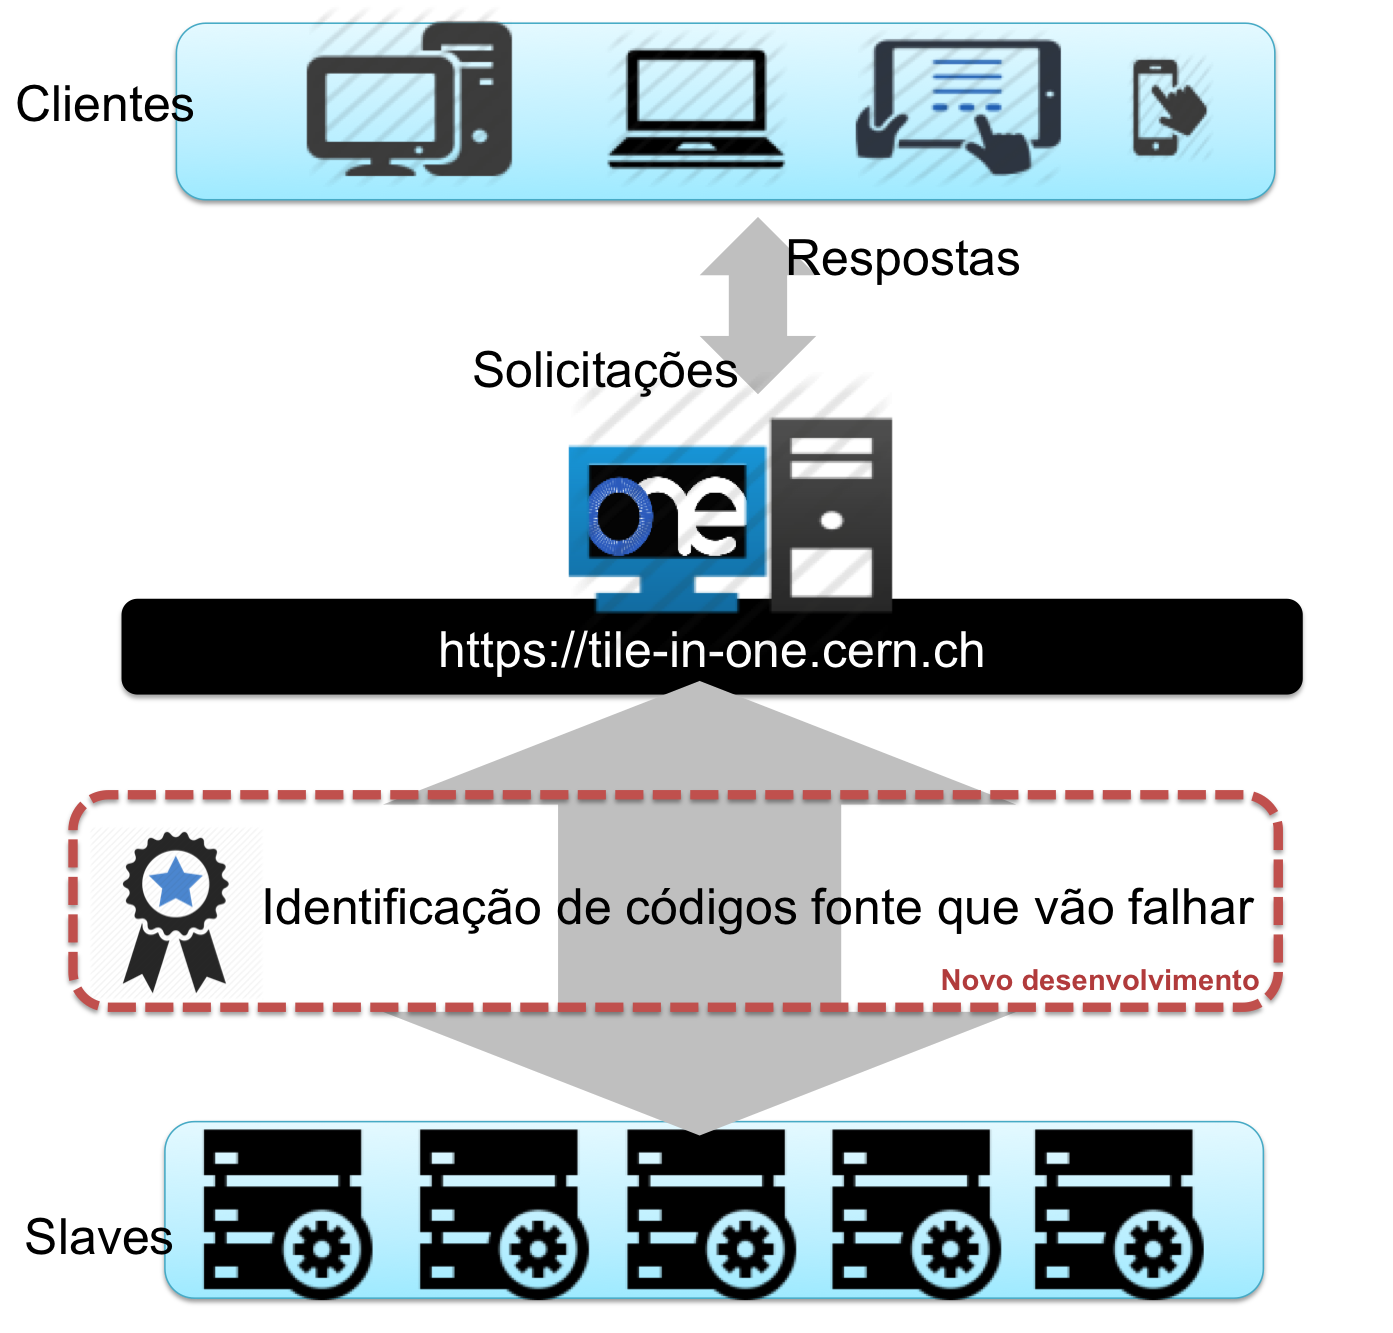
\includegraphics[width=8cm]{images/infrastructure.png}
      \caption{Esquem�tico representando a infraestrutura da plataforma Tile-in-ONE. Em vermelho, a nova camada a ser desenvolvida.}
      \label{fig:infrastructure}
    \end{figure}

    \section{Novo desenvolvimento}

    A plataforma Tile-in-ONE est� atualmente sendo utilizada pelos grupos de calibra��o e qualidade de dados do TileCal. Uma preocupa��o que surgiu ao longo do ano de 2014 foi a execu��o bem sucedida de c�digos fonte sem avalia��o pr�via. Cada c�digo que enfrenta falhas durante sua execu��o na m�quina \emph{slave} acaba consumindo recursos computacionais que podem comprometer o fluxo de dados da plataforma como um todo. A solu��o para tal quest�o levantada � estudada neste mestrado, fazendo uso de t�cnicas de minera��o de c�digos fonte, como abordado no cap�tulo~\ref{code_mining}.

    \begin{figure}[H]
      \centering
      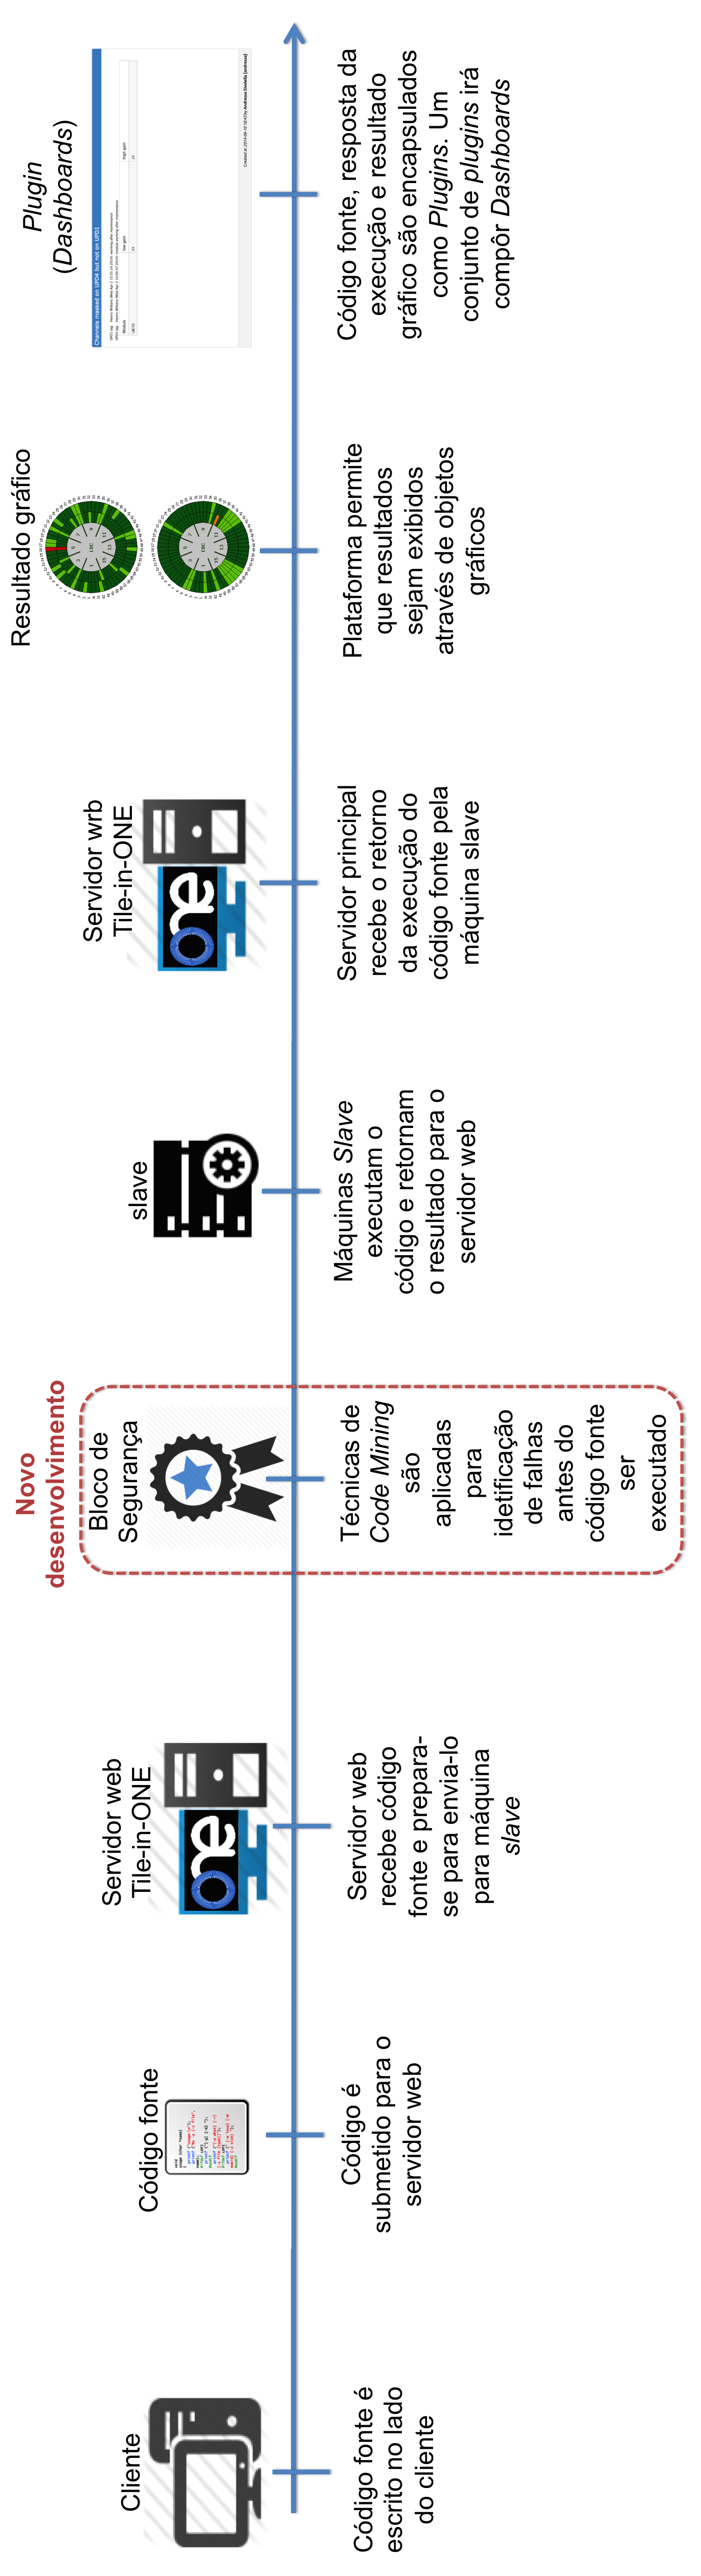
\includegraphics[width=7.5cm, height=24cm]{images/Tile-in-one_dataflow.png}
      \caption{Fluxo de dados da plataforma web Tile-in-ONE.}
      \label{fig:dataflow}
    \end{figure}
  \chapter{Minera��o de c�digos fonte para identifica��o de falhas}
\label{code_mining}
Em desenvolvimento de software � comum observar que quanto maior for o tempo de perman�ncia de um erro no c�digo mais custosa torna-se a sua corre��o e manuten��o em um projeto~\cite{IEEE-Software-McConnel}. Falhas em c�digos fonte s�o definidas como ``Imperfei��es durante o desenvolvimento de software que como consequ�ncia impedem que o programa atinja as expectativas desejadas."~\cite{BASKARAN2010}. Entende-se ainda que muitos defeitos s�o introduzidos durante o processo de desenvolvimento como um todo, n�o somente no seu in�cio ou fim. Assim sendo, identificar falhas antecipadamente torna-se parte essencial em desenvolvimento de software, que significa qualidade na entrega final do produto.~\cite{ODC1992}.

O SDLC (do ingl�s, \emph{software development life cycle} ou ciclo de vida do desenvolvimento de software)~\cite{6906040} indica que o desenvolvimento de software pode ser descrito em cinco etapas:
\begin{enumerate}
  \item{Levantamento de Requisitos}
  \item{Projeto}
  \item{Implementa��o}
  \item{Teste}
  \item{Implanta��o}
\end{enumerate}

A figura~\ref{fig:bug_insertion} ilustra em quais etapas do ciclo de vida de desenvolvimento do software s�o inseridos. Entidades presentes na �rea de engenharia de computa��o (tais como a IBM~\cite{IBM} e HCL~\cite{HCL}) confirmam que cerca de 35\% das falhas identificadas em c�digos fonte s�o inseridas na fase de implementa��o~\cite{CODEMINING2015}.

\begin{figure}[h]
  \centering
  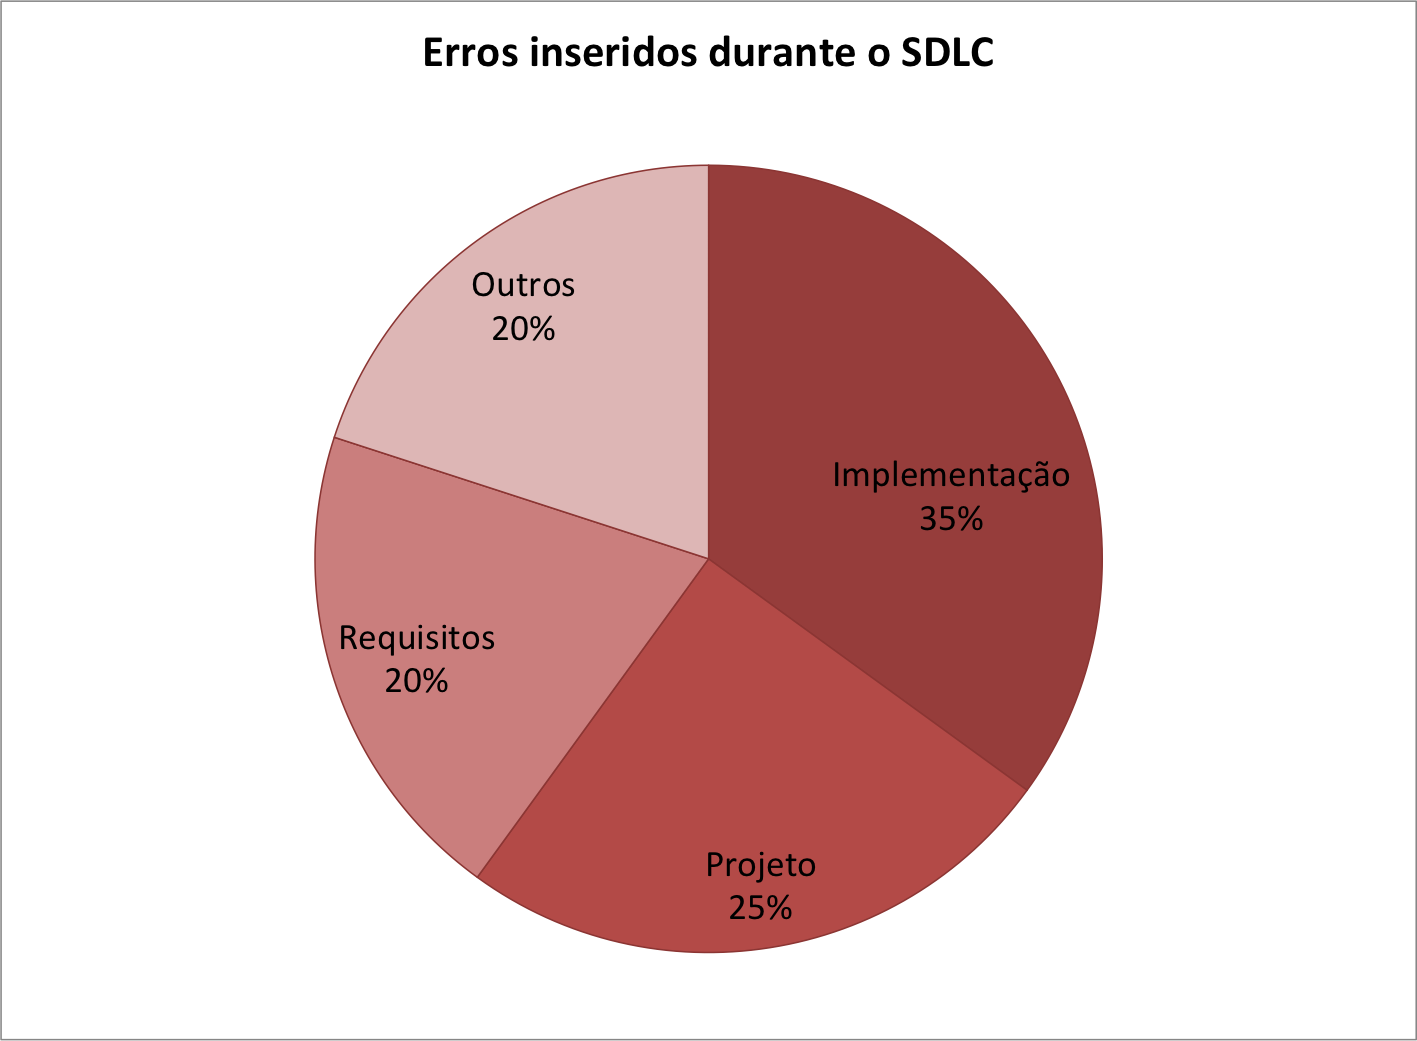
\includegraphics[width=8cm]{images/bug_insertion_sdlc.png}
  \caption{Estimativa do percentual de erros inseridos durante fases do SDLC. (Fonte: \emph{Computer Finance Magazine}. Dados extra�dos de~\cite{CODEMINING2015})}
  \label{fig:bug_insertion}
\end{figure}

Atualmente, diferentes t�cnicas tem sido utilizadas para identifica��o antecipada de erros em c�digos fonte. A an�lise est�tica, por exemplo, � bastante utilizada na �rea de programa��o desde a d�cada de 80. As caracter�sticas desta an�lise s�o abordadas em~\ref{static_analysis}. Em conjunto com analisadores est�ticos, pode-se aplicar t�cnicas de minera��o de dados, fazendo uma combina��o entre a �rea de engenharia de software e intelig�ncia computacional. No artigo~\cite{4222731}, publicado em 2007, os autores abordam como a minera��o de dados pode contribuir com a �rea de engenharia de software, a medida que t�cnicas de intelig�ncia computacional, quando aplicadas, melhoram a qualidade de projetos. Nesta mesma dire��o, a MSR (em ingl�s, \emph{Mining Software Repositories} ou minera��o de reposit�rios de c�digos) passa a ser amplamente abordada devido a disponibilidade gratuita de in�meros reposit�rios p�blicos de controle de versionamento, rastreamento de erros inseridos e at� mesmo documenta��es~\cite{4659248}.

Aplicar minera��o de dados em c�digos fonte desperta interesse na comunidade cient�fica, uma vez que c�digos s�o tipicamente estruturados e semanticamente ricos em termos de construtores de programa��o (tais como vari�veis, fun��es, objetos estruturados e rotinas bem definidas). Os objetivos s�o diversos: v�o desde a tentativa de descobrir o que um determinado software faz (sem necessariamente execut�-lo) at� manuten��o de projetos ou an�lises de desenvolvimento~\cite{130589}.

Como citado, a identifica��o antecipada de erros inseridos durante a implementa��o de c�digos fonte � atraente do ponto de vista de qualidade de produto. A utiliza��o de minera��o de c�digos � uma das aplica��es mais ativas em engenharia de software atualmente. Neste caso, o objetivo � obter ferramentas que n�o s� identifiquem falhas (ou \emph{bugs}) mas tamb�m sua localiza��o exata nas linhas de c�digos do projeto, de tal forma que o seu conserto seja facilitado~\cite{130589}. Para alcan�ar esse objetivo, uma dire��o de bastante destaque consiste na minera��o de padr�es, que uma vez pr�-definidos, s�o aplicadas em diversos reposit�rios de projetos j� existentes com o objetivo de encontrar anomalias comuns que violam regras (~\cite{Li05pr-miner:automatically},~\cite{4222586},~\cite{Chang:2007:FWN:1273463.1273486}).

Outro objetivo dominante na minera��o de c�digos � a tentativa de identificar fragmentos clonados. A n�o reutiliza��o de c�digos dificulta a manuten��o do software e ainda, pode proliferar \emph{bugs} em diferentes partes de um projeto.

A se��o~\ref{code_mining_cern} investiga a aplica��o de minera��o de dados em c�digos fonte no CERN; A se��o~\ref{categories} aborda quais s�o os atributos comumente utilizados quando minera��o de dados � aplicada em c�digos fonte. Esta se��o � composta por duas sub-se��es (~\ref{static_analysis} e~\ref{halstead}) que abordam em que situa��es tais atributos foram utilizados na aplica��o de minera��o de c�digos neste contexto;  Por fim, a se��o~\ref{ensemble} descreve m�todos de aprendizado de m�quina que foram utilizados neste mestrado na tentativa de classificar de c�digos fonte em \emph{execut�veis/n�o execut�veis}.

\section{Analisadores est�ticos e Minera��o de c�digos no CERN}
    \label{code_mining_cern}
    O CERN oferece um ambiente para desenvolvimento de software bastante particular. Estima-se que centenas de projetos de software est�o sendo desenvolvidos, com prop�sitos espec�ficos, desde programas que auxiliam o trabalho da equipe de recursos humanos at� os que monitoram o desempenho dos diversos experimentos do colisor de part�culas. Apesar do setor de TI do CERN ter estipulado algumas regras para a pol�tica de seguran�a, muitos projetos de software pequenos n�o as seguem a risca. Isso implica em vulnerabilidades de programas utilizados em ambientes de produ��o no CERN.

    As regras de seguran�a estipuladas n�o s�o t�o r�gidas para estimular o meio acad�mico no avan�o das pesquisas cient�ficas. Da mesma maneira, analisadores est�ticos para assegurar a qualidade no desenvolvimento de c�digos livres n�o s�o impostos para a comunidade presente. Existem ferramentas dispon�veis e com documenta��o e suporte da equipe de TI, mas nenhum projeto � obrigado a utiliz�-las. No caso deste projeto de mestrado, a linguagem computacional utilizada � o Python, sendo o \emph{PyLint}~\cite{pylint} uma ferramenta de an�lise est�tica cuja utiliza��o � incentivada pelo CERN~\cite{cern_recomendations_tools}.

    Recentemente, o setor de seguran�a em computa��o do CERN contratou um servi�o (\emph{Coverity}~\cite{Bessey:2010:FBL:1646353.1646374}) para garantir qualidade no desenvolvimento de novas funcionalidades no seu principal produto de an�lises f�sicas (o ROOT~\cite{BRUN}). O ROOT � utilizado por cerca de 10.000 pesquisadores e a integridade do software passou a ser vista como algo valioso. Um \emph{bug} perpetuado no ROOT pode ter um impacto muito negativo nas an�lises de resultados dos dados gerados pelo LHC. Assim que incorporado, o \emph{Coverity} j� foi capaz de identificar mais de 40.000 falhas em aproximadamente 50 milh�es de linhas de c�digos~\cite{coverity_numbers}. Um ponto negativo observado por desenvolvedores do ROOT � o tempo necess�rio para executar o analisador est�tico: s�o 28 horas para cada 2 milh�es de linhas de c�digo. � v�lido observar que a ferramenta escolhida para o ROOT n�o atende as necessidades deste projeto de mestrado: o \emph{Coverity} atende c�digos escritos em linguagem C/C++ enquanto os c�digos do Tile-in-ONE (se��o~\ref{tio}) s�o implementados em Python. Al�m disso, deseja-se aplicar minera��o de dados em c�digos fonte em um ambiente web.

    Em f�sica de altas energias n�o existem artigos que indiquem a aplica��o de minera��o de dados em c�digos fonte.


    \section{Escolha de atributos}
    \label{categories}
    Uma revis�o feita por Heckman~\cite{Heckman:2011:SLR:1945085.1945215} com 21 artigos sobre minera��o de dados em c�digos fonte, identifica cinco categorias comumente utilizadas como atributos:
    \begin{enumerate}
      \item{\emph{Alert Characteristics} (AC): abordagem que leva em considera��o os alertas gerados por analisadores est�ticos (sub-se��o~\ref{static_analysis});}
      \item{\emph{Code Characteristics} (CC): abordagem que considera medidas estat�sticas e de qualidade do c�digo fonte como atributos de entrada para algoritmos de m�quina de aprendizado(sub-se��o~\ref{halstead});}
      \item{\emph{Source code repository metrics} (SCR): atributos retirados de reposit�rios de c�digos. Nesta abordagem, leva-se em considera��o versionamentos (hist�rico de \emph{bugs} inseridos no projeto), coment�rios de atualiza��es e documenta��o sobre requisitos por exemplo;}
      \item{\emph{Bug database metrics} (BDM): Neste caso, existe uma base de dados para o projeto contendo todos as falhas j� surgidas e consertadas. O objetivo dessa abordagem � identificar padr�es que podem voltar a acontecer no projeto;}
      \item{\emph{Dynamic analyses metric} (DA): esta abordagem armazena resultados obtidos com an�lise din�mica de c�digos, mediante diversas execu��es (ver se��o~\ref{static_analysis})}.
    \end{enumerate}

    Tais categorias s�o descritas detalhadamente em~\cite{Heckman:2008}.

    Este mestrado utiliza as duas primeiras abordagens, descritas nas pr�ximas sub-se��es.

        \subsection{Analisadores Est�ticos}
        \label{static_analysis}

        Em engenharia de software existem dois tipos de an�lise (complementares) que podem ser feitas para validar e testar o produto em concep��o~\cite{1646907}:
        \begin{itemize}
          \item{\textbf{Est�tica}: neste caso apenas a estrutura do c�digo � analisada, mas o c�digo n�o � executado;
          }
          \item{\textbf{Din�mica}: para esta an�lise, � preciso levantar um plano de testes, execut�-los e avaliar os resultados. Ou seja, � necess�rio executar o c�digo diversas vezes;
          }
        \end{itemize}

        Como o objetivo deste mestrado � analisar c�digos fonte sem execut�-los,  utilizar analisadores est�ticos torna-se atraente, por defini��o.

        Na d�cada de 80, diversas ferramentas que aplicam an�lise est�tica de c�digo come�aram a ser desenvolvidas para auxiliar desenvolvedores na implementa��o de c�digos com menos \emph{bugs}~\cite{Tischler:1983:SAP:1006140.1006182}. Mas logo um inconveniente surge~\cite{YukselS13}: a quantidade de alertas gerados pelas ferramentas de an�lise est�tica de c�digo (SCAT, do ingl�s, \emph{Static Code Analysis Tools}) � grande e muitos deles n�o s�o acion�veis. Diz-se acion�vel um alerta que realmente vai impedir o sucesso na execu��o de um determinado c�digo. Essa classifica��o � feita manualmente pelo desenvolvedor (que neste caso � o especialista): se o especialista entende que determinado alerta � importante e precisa ser consertado antes da execu��o do programa, tal alerta � definido como \emph{acion�vel}. Caso contr�rio, ele � definido como \emph{n�o acion�vel}(~\cite{4815348},~\cite{Heckman:2008:EBE:1414004.1414013}).

        Empiricamente, existem cerca de 40 alertas para cada mil linhas de c�digo (KLOC, do ingl�s, \emph{Kilo Lines of Code})~\cite{Heckman:2008:EBE:1414004.1414013}. Desta estimativa, podem ser n�o acion�veis 30-100\%, como observado em~\cite{Aggarwal:2006:ISD:1169228.1170032},~\cite{4026864},~\cite{Heckman:2008:EBE:1414004.1414013},~\cite{4228664},~\cite{Kim:2007:WIF:1287624.1287633},~\cite{Kremenek:2003:ZUS:1760267.1760289}. Tais n�meros desestimulam desenvolvedores e projetistas a aplicar ferramentas de an�lise est�tica de c�digo no processo de desenvolvimento de software, embora entende-se a sua import�ncia no quesito qualidade adquirida. Por outro lado, um alerta definido pelo especialista como \emph{acion�vel} nem sempre vai impedir a execu��o bem sucedida do c�digo. Ou seja, se por um lado os analisadores est�ticos geram muitos alertas (\emph{n�o acion�veis}), nada garante que o alerta \emph{acion�vel} indica que o programa cont�m \emph{bugs} e vai falhar durante a tentativa de execu��o. Em outras palavras, um analisador est�tico pode n�o gerar nenhum alerta e mesmo assim, durante a tentativa de execu��o, o c�digo ainda pode falhar.

        Para este mestrado, um dos atributos utilizados corresponde a gera��o ou n�o de alertas pelo analisador est�tico. Adicionalmente, outras medidas estat�sticas e de qualidade, descritas a seguir, comp�em a lista inicial de atributos extra�dos de c�digos fonte(tabela~\ref{tab:initialattributes}).

        \subsection{Medidas estat�sticas e de qualidade}
        \label{halstead}

        Em computa��o, ``Halstead Metrics''~\cite{Halstead:1977:ESS:540137} s�o medidas de qualidade e estat�sticas definidas por Maurice Halstead e publicadas em 1977.

        As medidas estat�sticas (de Halstead) que podem ser extra�das de um c�digo fonte s�o:
        \begin{itemize}
          \item{$\eta_1$: quantidade de operadores distintos no c�digo;}
          \item{$\eta_2$: quantidade de operandos distintos no c�digo;}
          \item{$N_1$: total de operadores;}
          \item{$N_2$: total de operandos;}
        \end{itemize}

        Destas, outras medidas estat�sticas s�o tamb�m definidas por Halstead:
        \begin{itemize}
          \item{Vocabul�rio: $\eta = \eta_1 + \eta_2$;}
          \item{Tamanho: $N = N_1 + N_2$;}
          \item{Volume: $V = N log_2 \eta$;}
          \item{Dificuldade: $D = \frac{\eta_1}{2} . \frac{N_2}{\eta_2}$;}
          \item{Esfor�o: $E = D . V$;}
          \item{Estimativa de tempo de execu��o (em segundos): $ T = \frac{E}{18}$;}
          \item{Estimativa de potenciais \emph{bugs}: $ B = \frac{V}{3000} $};
        \end{itemize}

        Outra caracter�stica que pode ser extra�da de c�digos fonte � a sua complexidade. Define-se como ``Cyclomatic Complexity'' (do ingl�s, complexidade ciclom�tica)~\cite{maccabe1983structured} o n�mero de decis�es que um determinado bloco de c�digo cont�m mais uma unidade. Este n�mero (tamb�m conhecido como \emph{McCabe number}) representa o n�mero de caminhos independentes percorridos durante a execu��o de um c�digo, quando se monta uma �rvore abstrata de sintaxe (AST, do ingl�s, \emph{abstract syntax tree})~\cite{jones03pattern}.

        O �ndice de manutenabilidade (ou MI, do ingl�s \emph{Maintainability Index}) � uma medida em software que indica o qu�o f�cil � a manuten��o de um determinado c�digo. O MI � calculado de diferentes maneiras, dependendo da abordagem que se deseja utilizar. Entretanto, a f�rmula cl�ssica~\cite{242525} envolve o n�mero de linhas totais em um c�digo fonte (SLOC, do ingl�s, \emph{source lines of code}), a complexidade ciclom�tica (neste contexto, CC) e o volume de Halstead (HV): \\ $MI = 171 - 5.2 ln _{HV} - 0.23 _{CC} - 16.2 ln _{SLOC}$.\\Os autores chegaram nesta f�rmula atrav�s de um n�mero de c�digos fornecidos pela HP, escritos em linguagens de programa��o C e Pascal. Para cada c�digo, um especialista (engenheiro de software) atribuiu uma nota (de 1 a 100) indicando o qu�o f�cil seria fazer altera��es ou corre��es posteriores ao determinado c�digo (quanto maior a nota, mais f�cil � sua manuten��o). Consequentemente, 40 faixas de valores foram identificadas e atrav�s de uma regress�o estat�stica, eventualmente, a f�rmula exposta foi encontrada como um �ndice de manutenabilidade. Existe ainda o LLOC (do ingl�s, \emph{Logic Lines of Code}), que indica a quantidade de linhas com operadores l�gicos no c�digo e � outra medida que pode ser extra�da como um atributo de c�digos fonte.

        A tabela~\ref{tab:initialattributes} lista os atributos inicialmente extra�dos e uma breve descri��o. Uma an�lise de relev�ncia e correla��o foi realizada. Os resultados s�o apresentados na se��o~\ref{selection}.
        
    \begin{table}[]
    \centering
    \caption{Lista inicial de atributos}
    \label{tab:initialattributes}
    \begin{tabular}{@{}|l|c|l|@{}}
    \toprule
    \multicolumn{1}{|c|}{\textbf{\#}} & \textbf{Atributo}                       & \multicolumn{1}{c|}{\textbf{Descri��o}}                            \\ \midrule
    1                                 & Complexidade Ciclom�tica                & N�mero de declara��es                                              \\ \midrule
    2                                 & �ndice de Manutenabilidade              & Corresponde � organiza��o do c�digo                                \\ \midrule
    3                                 & Vocabul�rio de Hasltead                 & \# de operadores + \# de operandos �nicos                          \\ \midrule
    4                                 & Tamanho de Halstead                     & \# de operadores + \# total de operandos                           \\ \midrule
    5                                 & SLOC                                    & N�mero de linhas do c�digo fonte                                   \\ \midrule
    6                                 & \multicolumn{1}{l|}{Volume de Halstead} & Combina��o entre n�mero de linhas e declara��es                    \\ \midrule
    7                                 & Dificuldade de Hasltead                 & \begin{tabular}[c]{@{}l@{}}Complexidade do c�digo baseada no n�mero de \\ operadores e operandos\end{tabular} \\ \midrule
    8                                 & Tempo de Halstead                       & Tempo estimado para compilar um c�digo                             \\ \midrule
    9                                 & Bugs de Halstead                        & Possibilidade de bugs serem gerados                                \\ \midrule
    10                                & LLOC                                    & N�mero de linhas l�gicas                                           \\ \midrule
    11                                & Alertas PyLint                          & \begin{tabular}[c]{@{}l@{}}Verdadeiro se PyLint gerou alertas. \\ Caso contr�rio, falso\end{tabular}\\ \bottomrule
    \end{tabular}
    \end{table}

    \section{M�todos \emph{ensemble} em �rvores de Decis�o}
    \label{ensemble}
    �rvore de decis�o (DT, do ingl�s, \emph{Decision Tree})~\cite{Rokach:2008:DMD:1796114} � um algoritmo de aprendizado de m�quina supervisionado. O termo ``supervisionado'' indica que, durante a fase de treinamento, as classes (ou alvos) s�o conhecidas. Desta maneira, o classificador aprende com casos em que se sabe a resposta (\emph{execut�vel}/\emph{n�o execut�vel}).

    Basicamente, o treinamento de uma �rvore de decis�o divide e agrupa o conjunto de treino em dois ou mais grupos homog�neos, sucessivamente. Para as divis�es, o algoritmo se encarrega de escolher qual � o atributo mais significativo, ou seja, qual atributo ir� tornar a divis�o o mais homog�nea (ou pura) poss�vel. Tal processo consiste no que se conhece como \emph{splitting} e ser� descrito mais adiante nesta se��o.

    A figura[XXX] ilustra um exemplo cl�ssico de �rvore de decis�o. Ele representa uma �rvore que decide se uma pessoa vai ou n�o jogar t�nis. Os atributos utilizados s�o condi��es do tempo (ensolarado, nublado ou chuvoso), umidade (alta ou baixa) e vento (forte ou fraco).

    Ainda sobre a figura[XXX], o conhecimento de algumas nomenclaturas � necess�rio. Elas ser�o referenciadas mais adiante. S�o elas:
    \begin{itemize}
        \item{O n� raiz (em azul) representa todo o conjunto de treino e � onde as divis�es em grupos homog�neos come�a.}
        \item{Os n�s que continuam dividindo os sub-conjuntos restantes (em cinza) s�o denominados n�s de decis�o.}
        \item{Quando a divis�o cessa, tem-se folhas (em verde). As folhas indicam a decis�o tomada pela �rvore treinada.}
    \end{itemize}

    Existem duas opera��es relacionadas ao treinamento de �rvores de decis�o. Elas est�o descritas a seguir.\\ \\
    \textbf{\large{Splitting}}\\ \\
    \textbf{\large{Pruning}}\\

    Uma das vantagens em se utilizar �rvores de decis�o para classifica��o � a sua f�cil compreens�o. Para pessoas sem conhecimentos em intelig�ncia computacional, o treinamento de classificadores e os resultados obtidos s�o de f�cil compreens�o. Al�m disso, a representa��o gr�fica � intuitiva e permite que hip�teses sejam rapidamente relacionadas.

    Entretanto, existe uma desvantagem que faz com que �rvores de decis�o n�o sejam consideradas classificadores fortes: o fato de dividir conjuntos em sub-conjuntos homog�neos faz com que o classificador gerado fique especialista no conjunto de treino (\emph{overfit}). Ou seja, a �rvore gerada sempre depender� do conjunto de treino utilizado. O m�todo \emph{ensemble} contorna essa quest�o levantada.

    \emph{Ensemble} s�o conjuntos de classificadores que combinam seus resultados individuais (por vota��o ou m�dia ponderada) para classificar novas amostras~\cite{Seni:2010:EMD:1841412}. Uma das �reas mais ativas na �rea de aprendizado de m�quina supervisionado tem sido \emph{ensemble}~\cite{Dietterich:2000:EMM:648054.743935}. Geralmente, classificadores \emph{ensemble} apresentam maior acur�cia que classificadores individuais. A raz�o estat�stica para isso � que a vari�ncia de um somat�rio � menor que a vari�ncia individual. Computacionalmente, o treinamento pode dar-se de maneira mais r�pida, uma vez que, em alguns casos � poss�vel paralelizar a fase de treinamento.

    Classificadores \emph{ensemble} podem ser gerados com qualquer algoritmo base, inclusive �rvores de decis�o. Tais classificadores s�o descritos nas sub-se��es a seguir.

    \subsection{Bagged Trees (\emph{\textbf{B}ootstrap \textbf{Agg}regating})}
    \label{bagged}

    Apesar do nome, \emph{Bagged Trees} pode ser utilizado com qualquer algoritmo base. Neste tipo de \emph{ensemble}, um sub-conjunto com N elementos do conjunto de treino � selecionado para o treinamento de um classificador. Em seguida, um novo sub-conjunto com outros N elementos � utilizado para gerar um outro classificador. Esse procedimento � repetido, at� que um n�mero total e pr�-definido de classificadores seja gerado. A classifica��o final d�-se por voto majorit�rio. A figura~\ref{fig:bagged_pseudocode} ilustra um pseudo-c�digo que descreve como \emph{Bagged Trees} � treinado e utilizado para classifica��es.

    \begin{figure}[htbp]
      \centering
        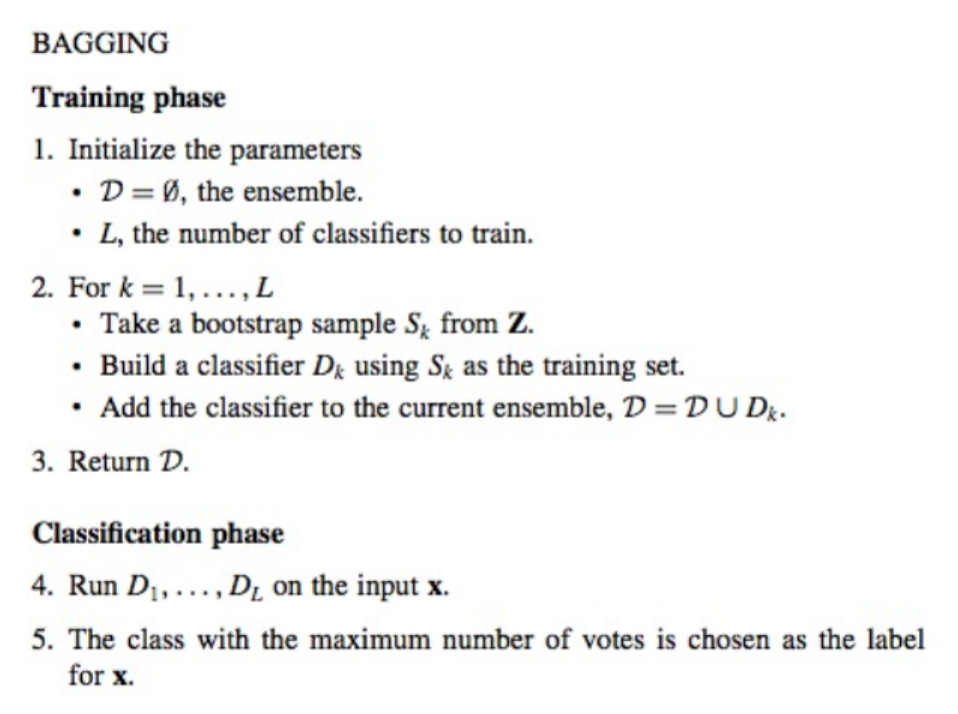
\includegraphics[width=9.0cm]{images/bagged_pseudocode.png}
        \caption{\emph{Bagged Trees} pseudo-c�digo. Retirado de ~\cite{Rokach:2008:DMD:1796114}.}
      \label{fig:bagged_pseudocode}
    \end{figure}

    \subsection{Random Forest}
    \label{randomforest}
    Alguns autores consideram \emph{Random Forest} como uma varia��o de \emph{Bagged Trees}~\cite{Dietterich:2000:EMM:648054.743935}. Este classificador \emph{ensemble} � apresentado por Breiman em~\cite{Breiman:2001:RF:570181.570182}.

    A primeira diferen�a � que \emph{Random Forest} s� utiliza �rvores de decis�o como algoritmo base. Outra diferen�a entre os dois algoritmos � a quantidade de atributos utilizados durante o treinamento dos classificadores: neste caso, nem todos os atributos s�o utilizados. Escolhe-se a quantidade de atributos que ser� utilizada e a cada nova �rvore, um sub-conjunto diferente de atributos � utilizado. Isso permite analisar a contribui��o de cada atributo no treinamento de cada �rvore.

    O termo \emph{Out of Bag (OOB)} tamb�m � introduzido por Breiman. Assim, tem-se uma nova medida para erro: cerca de um ter�o do conjunto de treino � separada e utilizada a cada rodada como um conjunto de teste. � a partir desta medida que a an�lise de contribui��o dos atributos torna-se poss�vel.

    Similar ao \emph{Bagged Trees}, o resultado final d�-se por voto majorit�rio.

    \subsection{Boosted Decision Trees (BDT)}
    \label{bdt}
    Este � outro algoritmo \emph{ensemble} que n�o exige apenas �rvores de decis�o como classificador base. Diferentemente dos casos anteriores, todo o conjunto de treino � utilizado para gerar o classificador. Mas, a cada rodada, verifica-se quais amostras foram erroneamente classificadas e atribui-se um peso a elas. Desta maneira, na pr�xima itera��o, os casos equivocados estar�o evidenciados. A figura~\ref{fig:bdt_example} ilustra o que ocorre com o conjunto de treino a cada rodada: dadas duas classes, verde e vermelha, ao gerar o primeiro classificador, temos 3 amostras erroneamente classificadas (\emph{misclassifieds}). Em outras palavras, temos 3 amostras que pertencem a classe verde, mas o classificador gerado atribuiu a classe vermelha a elas. Em uma pr�xima itera��o, tais amostras ser�o multiplicadas por um fator que influenciar� o treinamento. O resultado final ocorre por voto majorit�rio.

    � interessante observar na figura~\ref{fig:bdt_result} que a combina��o de diversos classificadores gera um classificador refinado.

    \begin{figure}[!ht]
    \centering
    \subfigure[Exemplo do que ocorre com o conjunto de treino durante as itera��es do BDT]{
      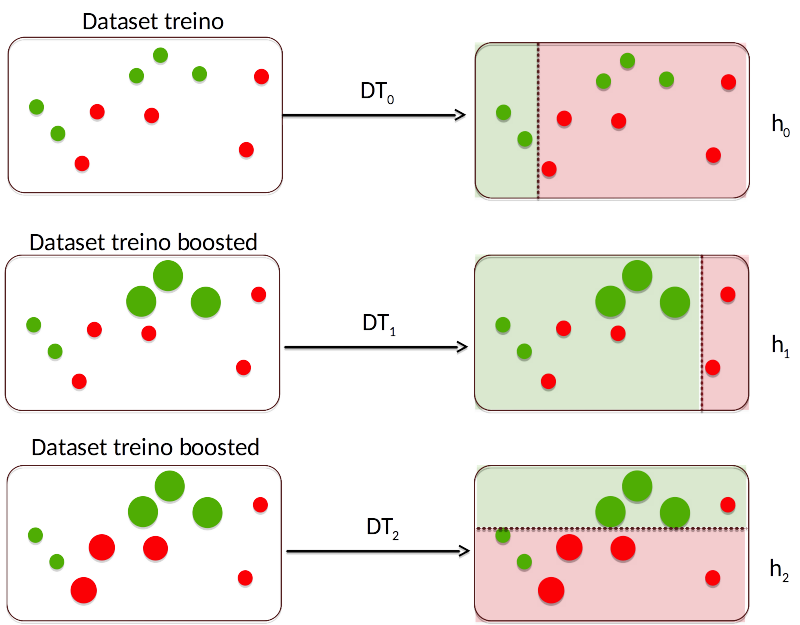
\includegraphics[width=8cm]{images/bdt_example.png}
      \label{fig:bdt_example}
    }
    \subfigure[O resultado final � por voto majorit�rio.]{
      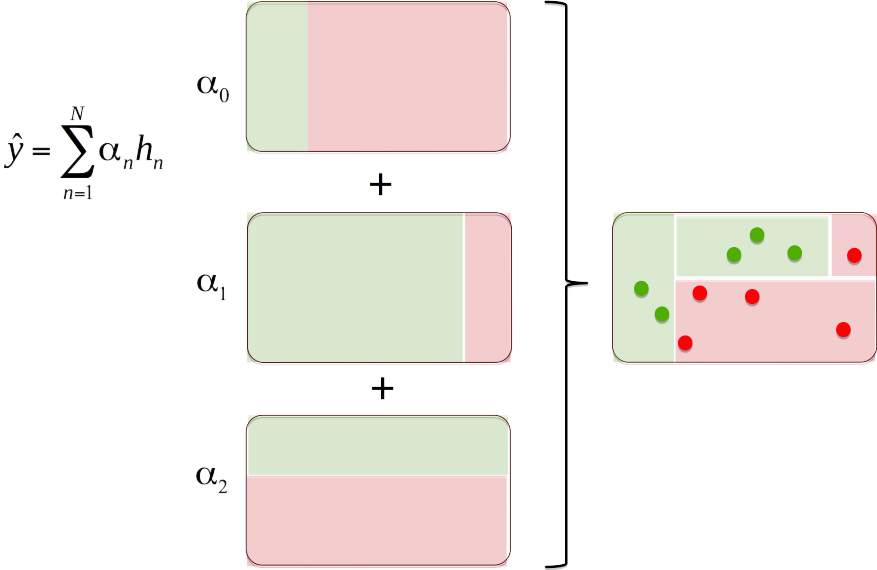
\includegraphics[width=8cm]{images/bdt_result.png}
      \label{fig:bdt_result}
    }
    \caption{Ilustra��o do m�todo BDT. Baseado em~\cite{Duda:2000:PC:954544}.}
    \label{bdt_training}
  \end{figure}

  \chapter{Metodologia}
\label{metodologia}
Este cap�tulo descreve o processo de estudo utilizado para este mestrado. 

As se��es~\ref{dataset} e~\ref{selection} descrevem, respectivamente, o conjunto de dados adquiridos e os atributos que foram previamente selecionados; A se��o~\ref{ensemble} descreve os algor�timos de m�quina de aprendizado utilizados;

    \section{Base de dados}
    \label{dataset}
    O Tile-in-ONE encontra-se em produ��o, sendo utilizado pelos grupos de calibra��o e qualidade de dados do TileCal desde 2014. Em seu banco de dados, existe um total de 512 c�digos de Plugins, desenvolvidos pelos colaboradores atrav�s da plataforma web. A figura~\ref{fig:developed_source_codes} corresponde a quantidade de c�digos fonte implementados no per�odo de Junho de 2014 a Dezembro de 2015.

    \begin{figure}[H]
      \centering
      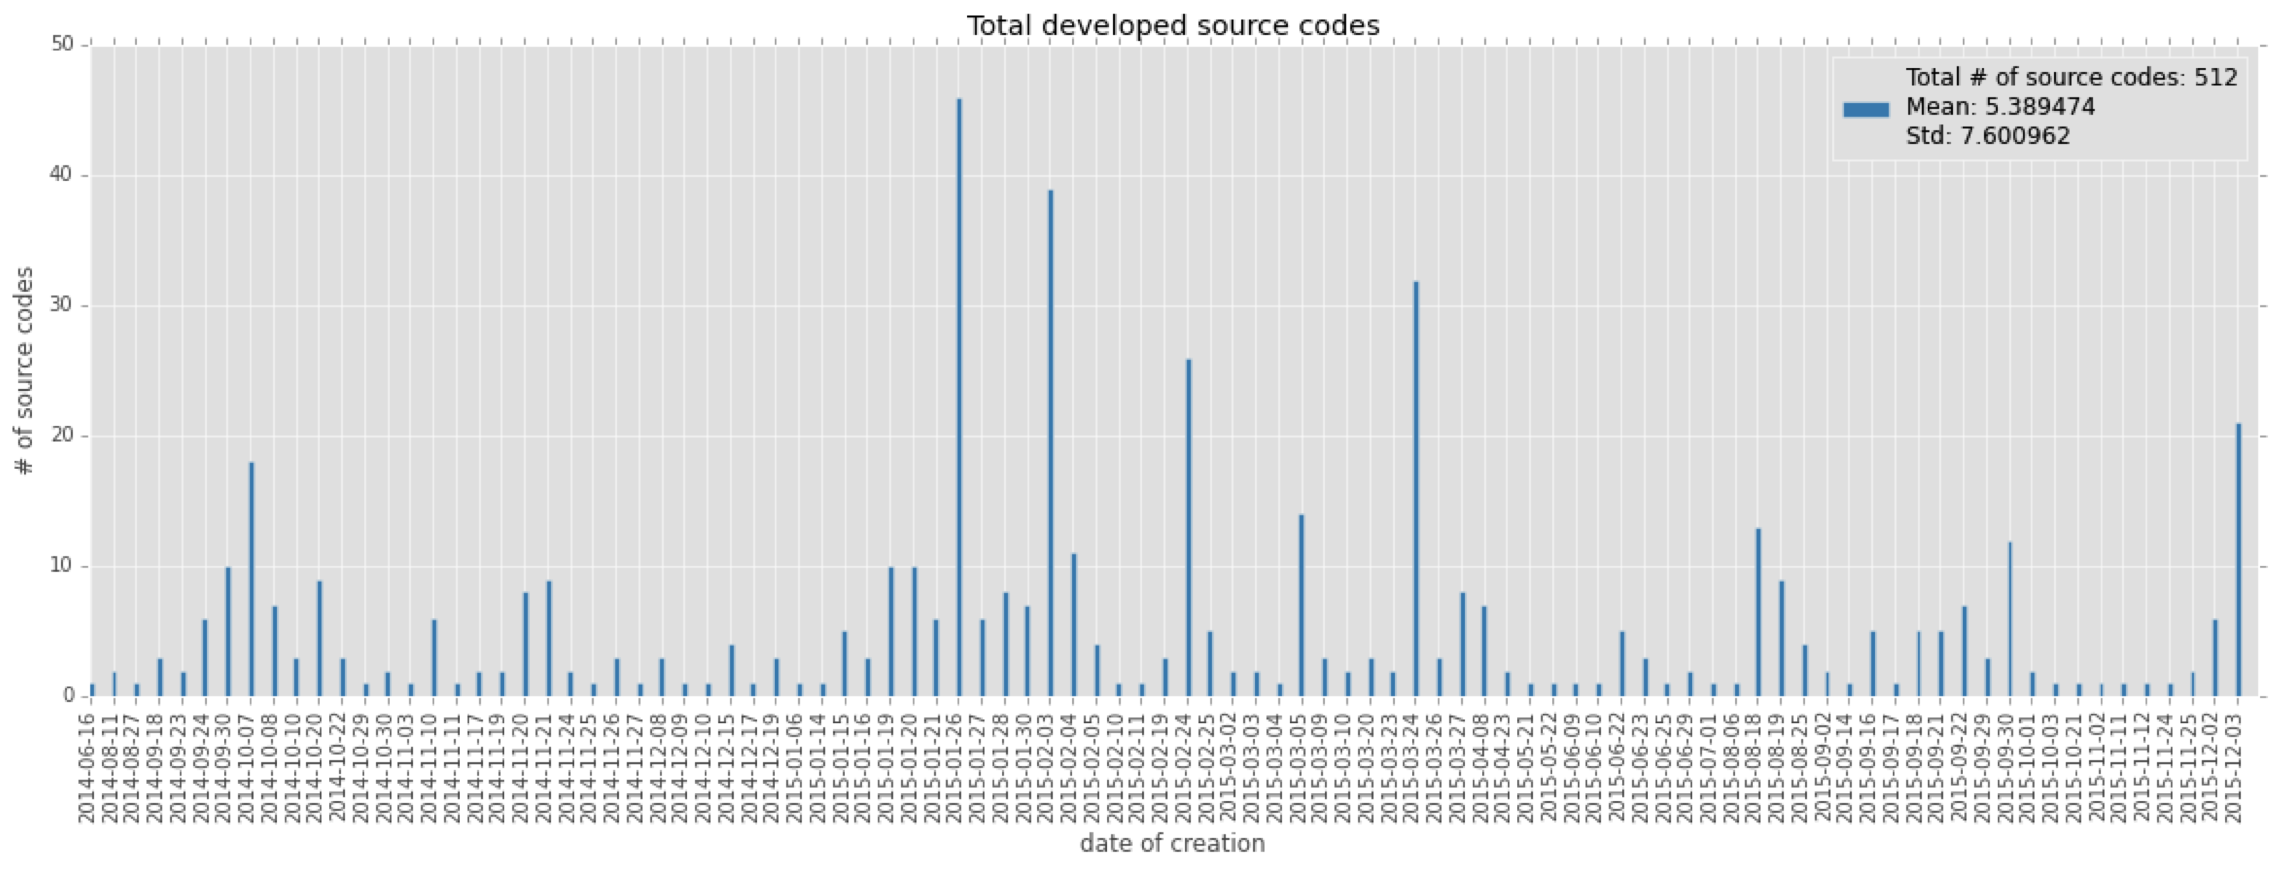
\includegraphics[width=17cm]{images/total_source_codes.png}
      \caption{Total de c�digos fonte escritos (512) entre Junho/2014 e Dezembro/2015.}
      \label{fig:developed_source_codes}
    \end{figure}

    Dos 512 c�digos que comp�em o conjunto de dados, quase 30\% n�o obtiveram sucesso ao serem enviados para uma m�quina \emph{slave}. De acordo com a figura~\ref{fig:slave_machine_results}, percebe-se que 8,59\% n�o retornaram nenhum tipo de resposta para o servidor principal, o que pode significar que a m�quina \emph{slave} escolhida para executar o c�digo fonte em quest�o estava sem comunica��o. Isso n�o significa necessariamente que o c�digo fonte � \emph{n�o execut�vel}, uma vez que ele nem sequer chegou na m�quina \emph{slave}. Os 21,09\% restantes correspondem a programas que falharam durante a tentativa de execu��o. Mas novamente, n�o � poss�vel afirmar neste momento que tais c�digos s�o \emph{n�o execut�veis}. Se por ventura, algum desses tentou acessar um banco de dados (externo a plataforma) que no momento da execu��o estava inacess�vel, a m�quina \emph{slave} retornou falha e, neste caso, o problema n�o foi o c�digo fonte. Talvez no futuro, esse tipo de informa��o possa se tornar uma entrada para o classificador: caso o c�digo fonte esteja acessando uma fonte externa ele pode ser penalizado.

    \begin{figure}[H]
      \centering
      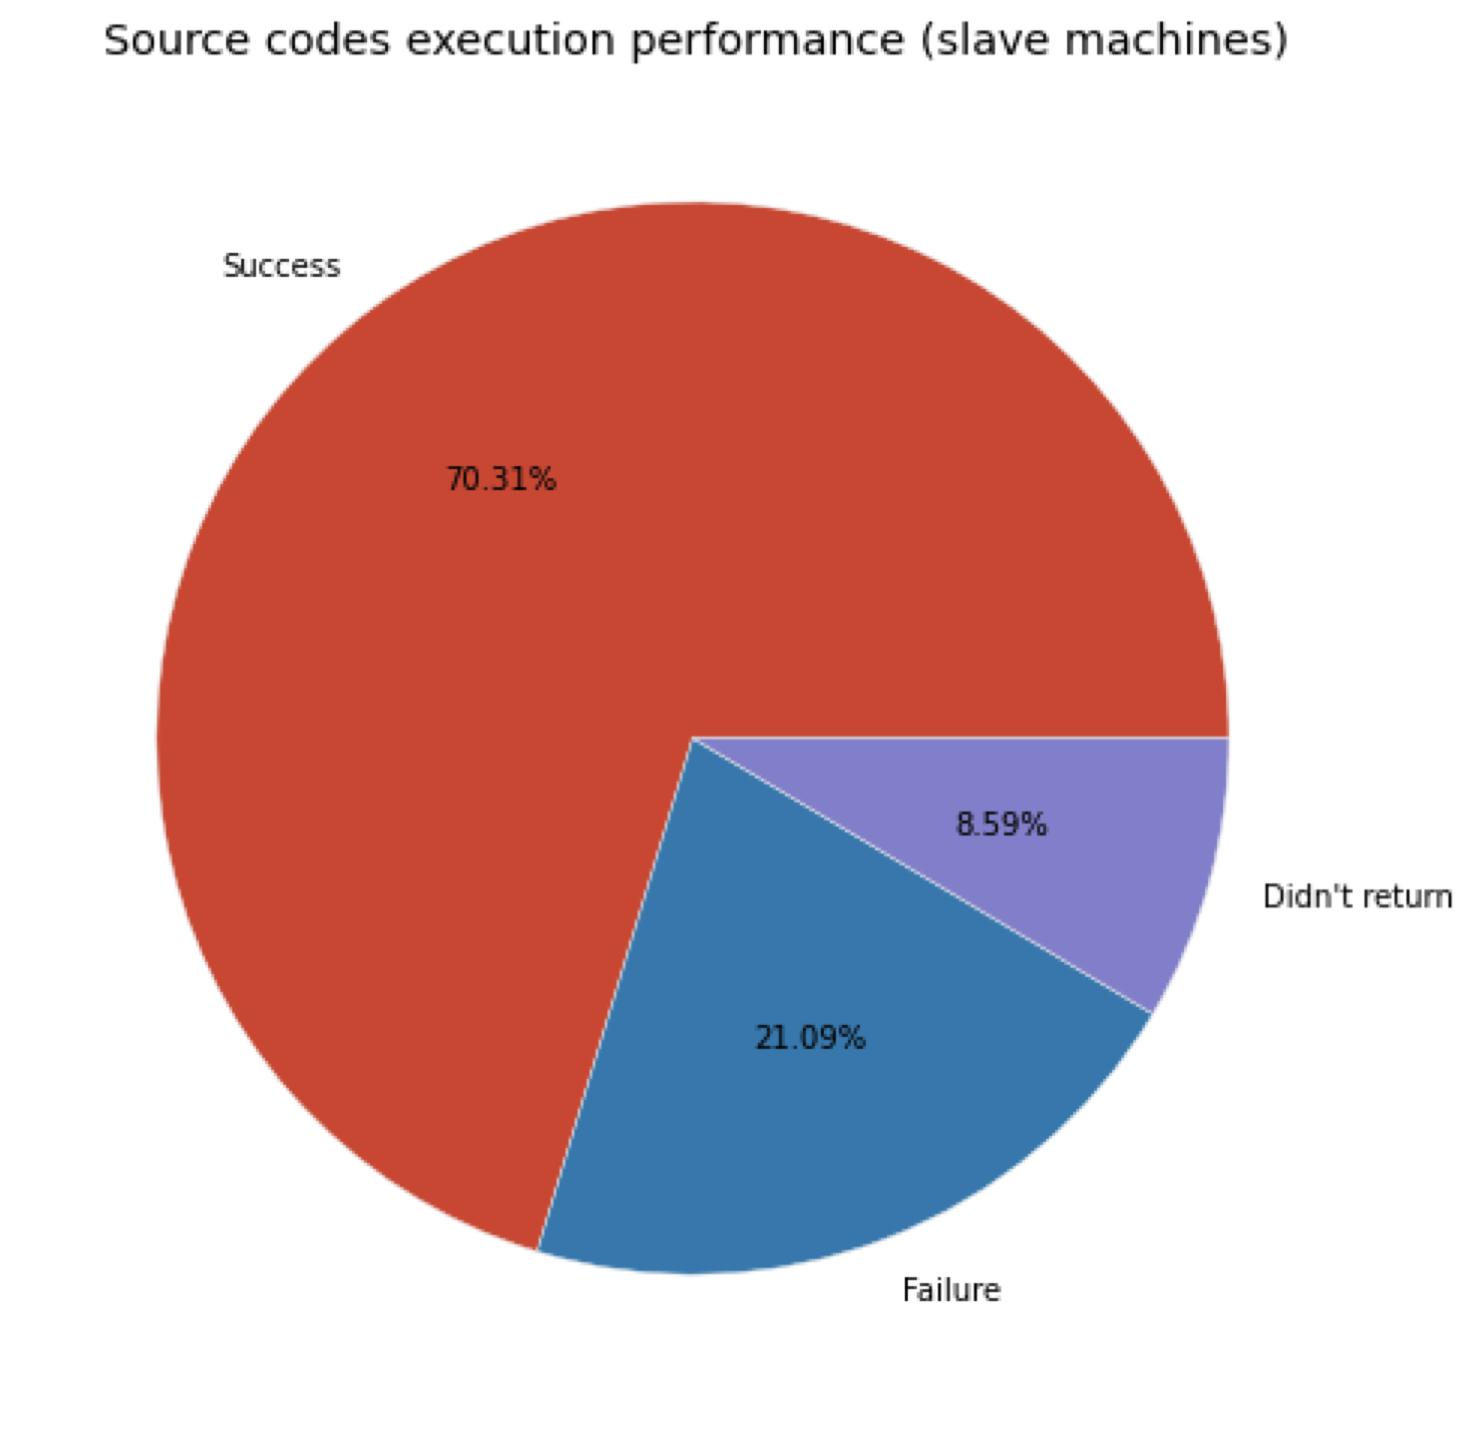
\includegraphics[width=8cm]{images/slave_machines_results.png}
      \caption{Retornos obtidos ap�s tentativa de executar c�digos fonte em m�quinas \emph{slave}.}
      \label{fig:slave_machine_results}
    \end{figure}

    Ap�s avaliar os 512 c�digos, e comparar com a aplica��o do analisador est�tico (PyLint), percebe-se que 82,02\% dos c�digos s�o \emph{execut�veis}, mas em quase 20\% dos casos o PyLint gera algum tipo de alerta. Do restante, menos de 1\% � \emph{n�o execut�vel} devido a erros de sintaxe em Python, mas podem ser facilmente identificados ao executar o analisador est�tico. Dos outros quase 17\% \emph{n�o execut�veis}, cerca de 5\% n�o podem ser identificados apenas com a aplica��o do Pylint. A figura~\ref{fig:targets} ilustra esses percentuais.

    \begin{figure}[H]
      \centering
      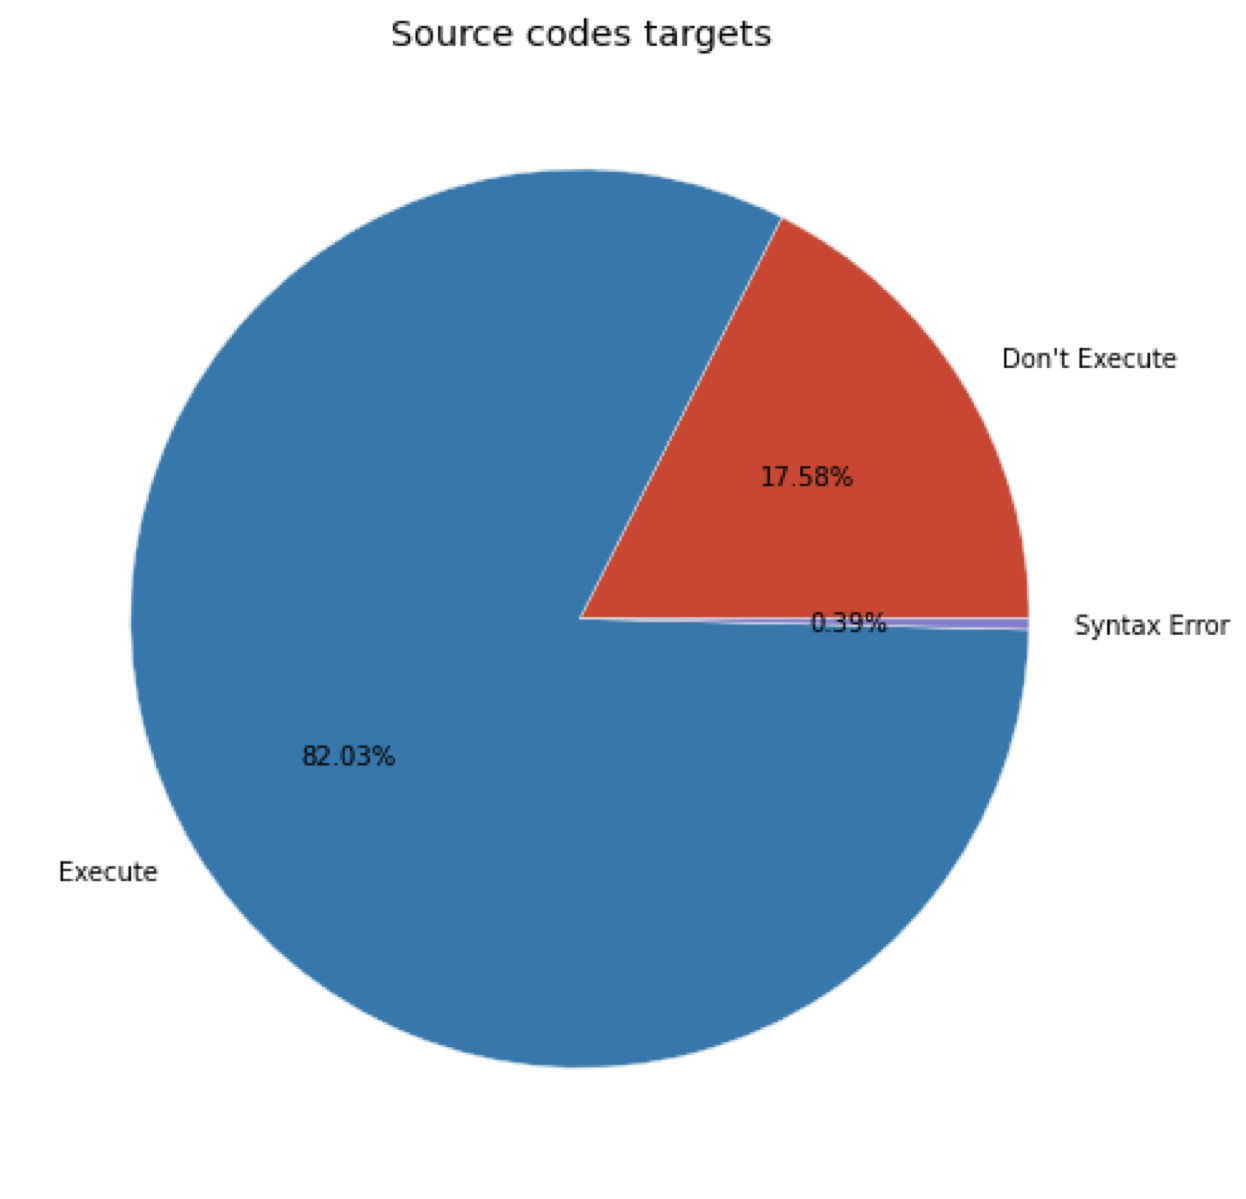
\includegraphics[width=8cm]{images/targets.png}
      \caption{Percentuais de alvos do conjunto de c�digos fonte.}
      \label{fig:targets}
    \end{figure}

    Em suma, a aplica��o do analisador est�tico n�o � suficiente para classificar um c�digo como \emph{execut�vel} ou \emph{n�o execut�vel}. Uma ferramenta adicional faz-se necess�ria.


    \section{Sele��o de categorias}
    \label{selection}

    \section{M�todos \emph{ensemble} em �rvores de Decis�o}
    \label{ensemble}                                                                                                                                                                                                                                                                                                                                                                          
  \chapter{M�todos utilizados e Discuss�o de resultados}
As se��es~\ref{dataset} e~\ref{selection} descrevem, respectivamente, o conjunto de dados adquiridos e os atributos que foram previamente selecionados.

Em seguida o cap�tulo apresenta uma discuss�o do desempenho obtido pelos classificadores \emph{ensemble}.
\section{Aquisi��o de c�digos fonte}
    \label{dataset}
    O Tile-in-ONE encontra-se em produ��o, sendo utilizado pelos grupos de calibra��o e qualidade de dados do TileCal desde 2014. Em seu banco de dados, foram selecionados para este projeto um total de 512 c�digos de \emph{Plugins}, desenvolvidos pelos colaboradores atrav�s da plataforma web. A figura~\ref{fig:developed_source_codes} ilustra a quantidade de c�digos fonte implementados no per�odo de Junho de 2014 a Dezembro de 2015.

    \begin{figure}[H]
      \centering
      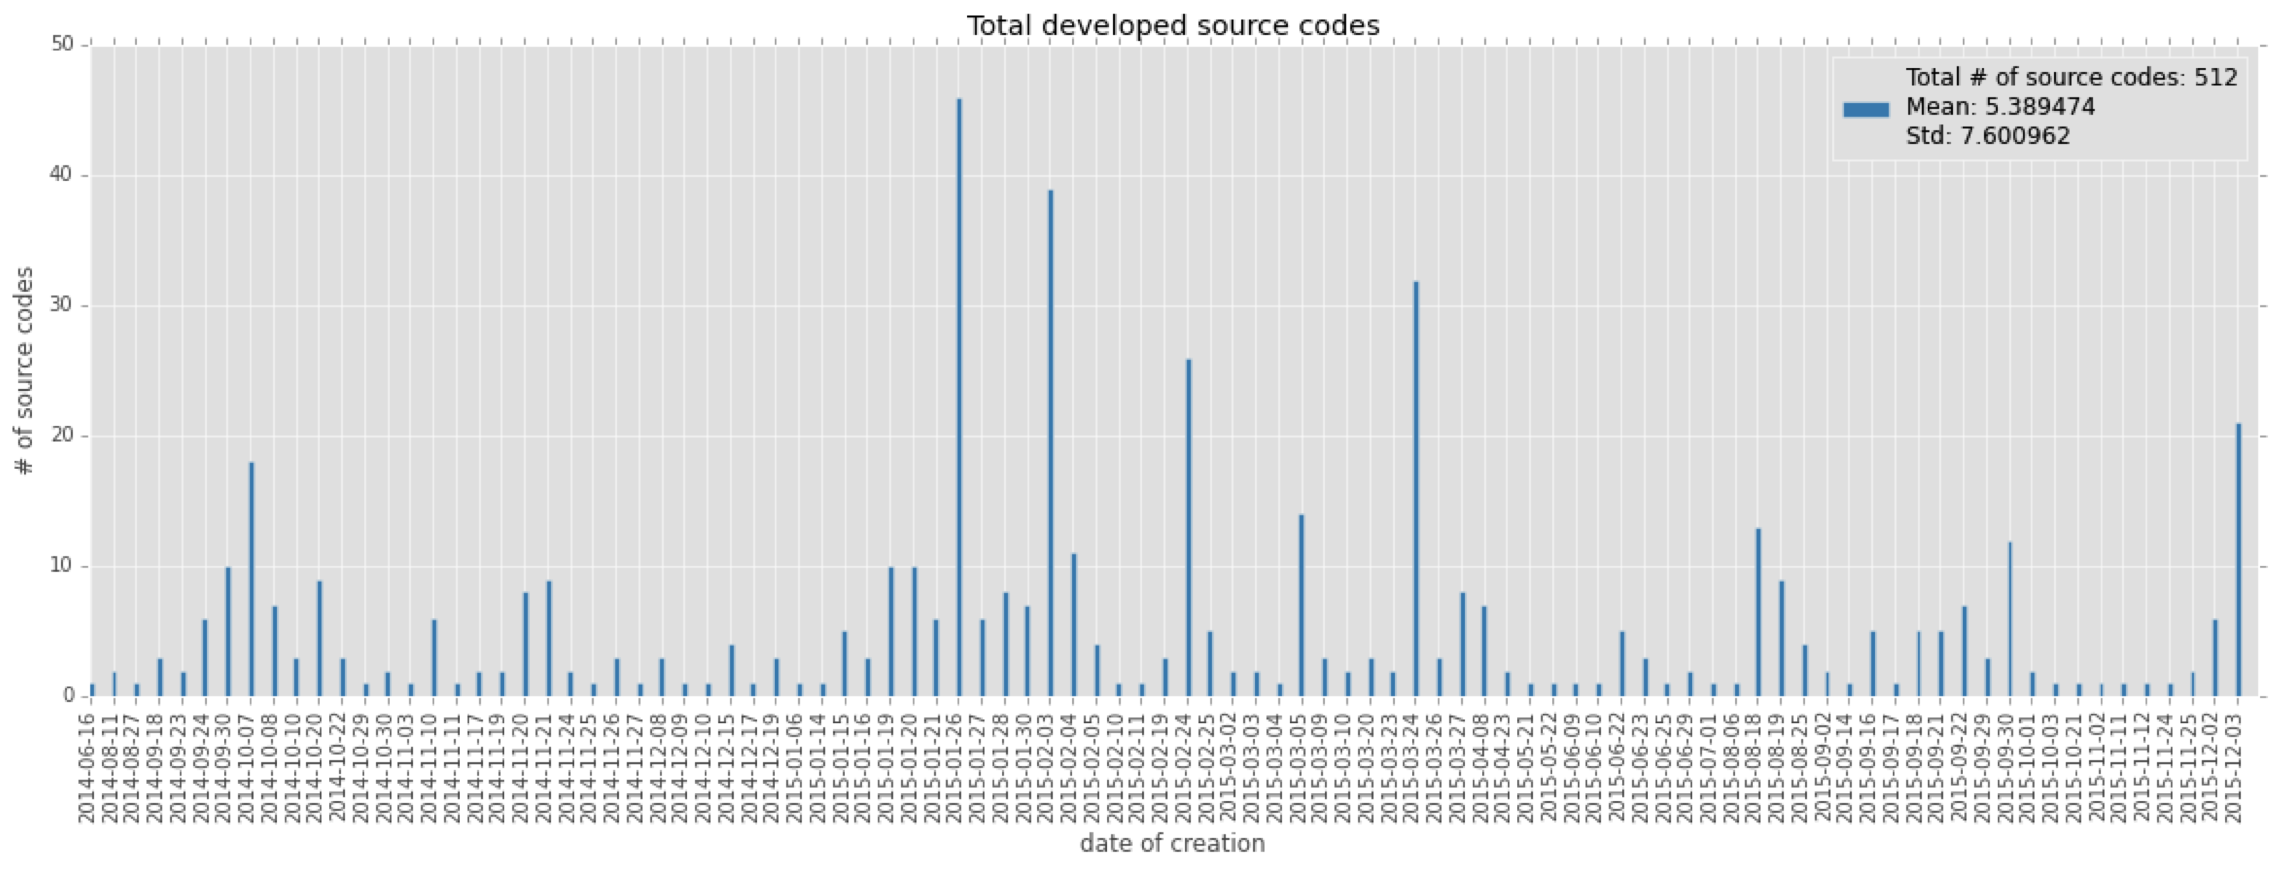
\includegraphics[width=17cm]{images/total_source_codes.png}
      \caption{Total de c�digos fonte escritos (512) entre Junho/2014 e Dezembro/2015.}
      \label{fig:developed_source_codes}
    \end{figure}

    Dos 512 c�digos que comp�em o conjunto de dados, quase 30\% n�o obtiveram sucesso ao serem enviados para uma m�quina \emph{slave}. De acordo com a figura~\ref{fig:slave_machine_results}, percebe-se que 8,59\% n�o retornaram nenhum tipo de resposta para o servidor principal, o que pode significar que a m�quina \emph{slave} escolhida para executar o c�digo fonte em quest�o estava sem comunica��o. Isso n�o significa necessariamente que o c�digo fonte � \emph{n�o execut�vel}, uma vez que ele nem sequer chegou na m�quina \emph{slave}. Os 21,09\% restantes correspondem a programas que falharam durante a tentativa de execu��o. Mas novamente, n�o � poss�vel afirmar neste momento que tais c�digos s�o \emph{n�o execut�veis}. Se por ventura, algum desses tentou acessar um banco de dados (externo a plataforma) que no momento da execu��o estava inacess�vel, a m�quina \emph{slave} retornou falha e, neste caso, o problema n�o foi o c�digo fonte. Talvez no futuro, esse tipo de informa��o possa se tornar uma entrada para o classificador: caso o c�digo fonte esteja acessando uma fonte externa ele pode ser penalizado.

    \begin{figure}[H]
      \centering
      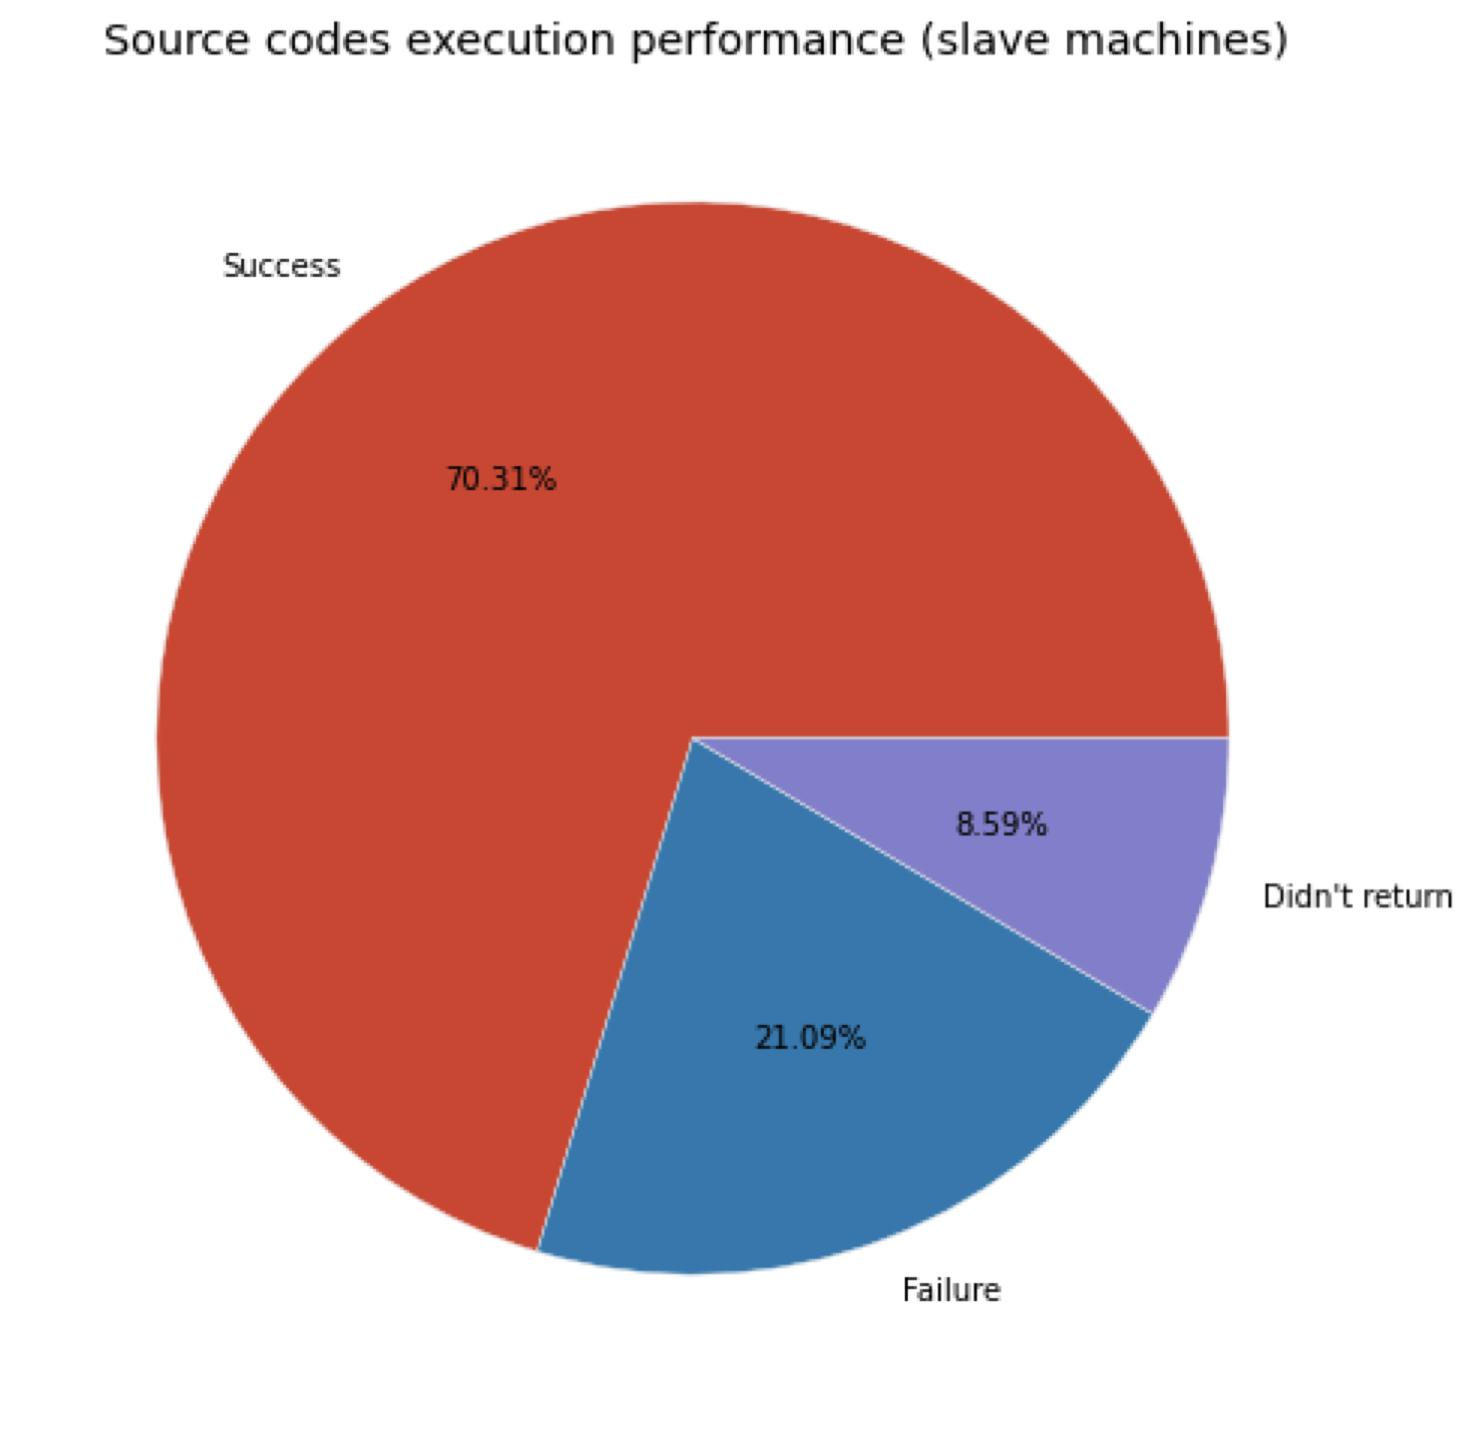
\includegraphics[width=8cm]{images/slave_machines_results.png}
      \caption{Retornos obtidos ap�s tentativa de executar c�digos fonte em m�quinas \emph{slave}.}
      \label{fig:slave_machine_results}
    \end{figure}

    Ap�s avaliar os 512 c�digos, e comparar com a aplica��o do analisador est�tico (PyLint), percebe-se que 82,02\% dos c�digos s�o \emph{execut�veis}, mas em quase 20\% dos casos o PyLint gera algum tipo de alerta. Do restante, menos de 1\% � \emph{n�o execut�vel} devido a erros de sintaxe em Python, mas podem ser facilmente identificados ao executar o analisador est�tico. Dos outros quase 17\% \emph{n�o execut�veis}, cerca de 5\% n�o podem ser identificados apenas com a aplica��o do Pylint. A figura~\ref{fig:targets} ilustra esses percentuais.

    \begin{figure}[H]
      \centering
      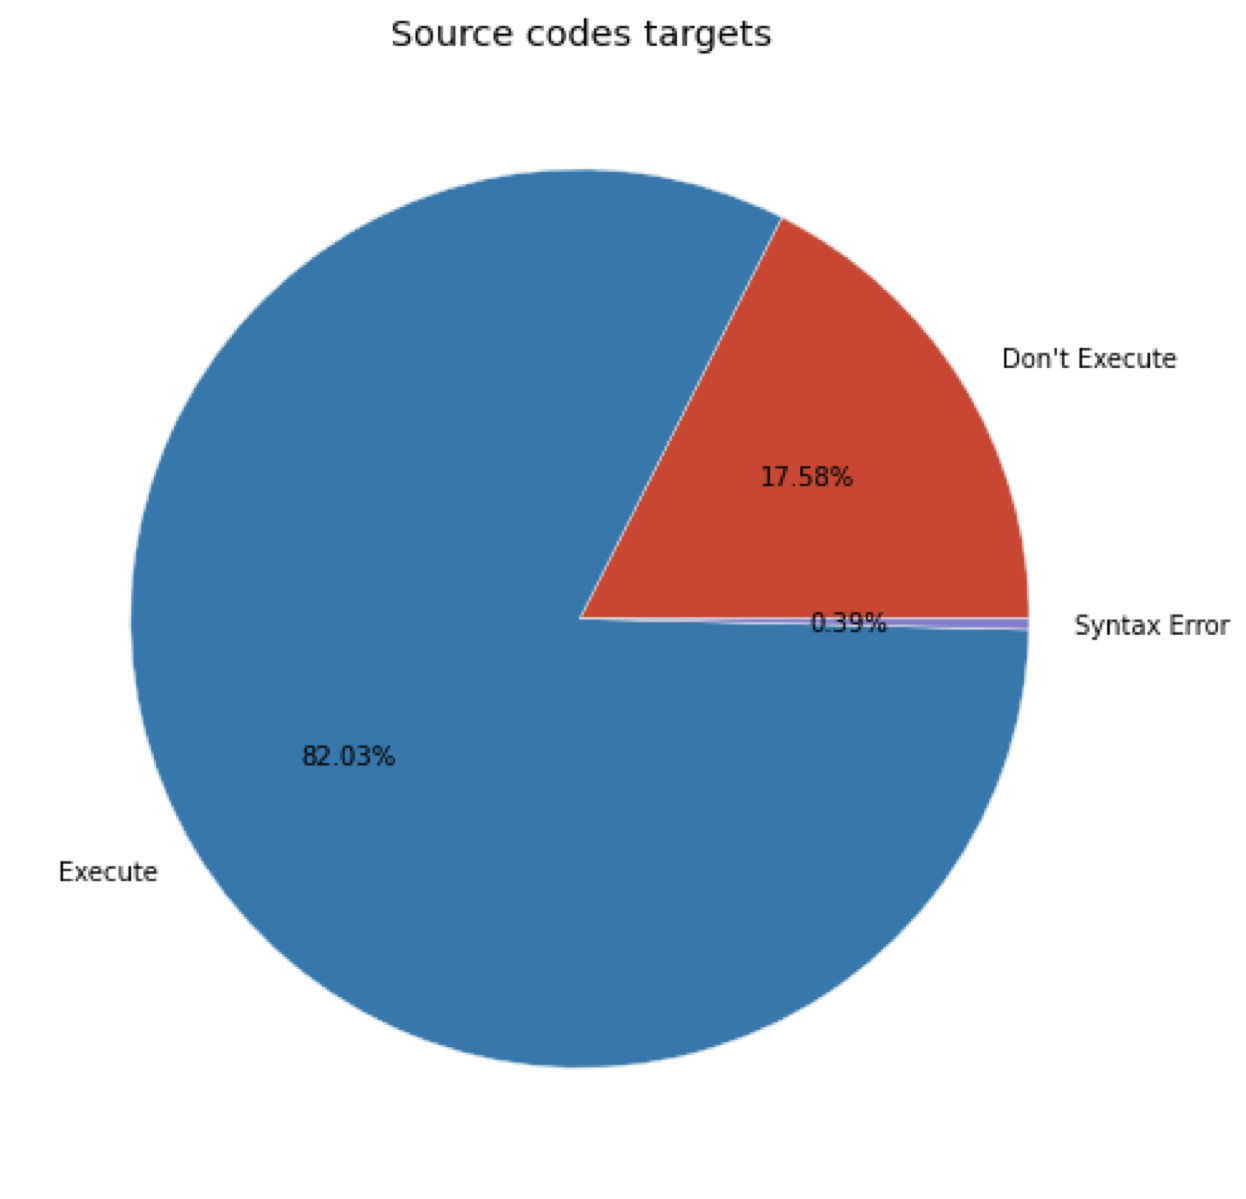
\includegraphics[width=8cm]{images/targets.png}
      \caption{Percentuais de alvos do conjunto de c�digos fonte.}
      \label{fig:targets}
    \end{figure}

    Em suma, a aplica��o do analisador est�tico n�o � suficiente para classificar um c�digo como \emph{execut�vel} ou \emph{n�o execut�vel}. Uma ferramenta adicional faz-se necess�ria.

    \section{An�lise de atributos}
    \label{selection}
    A tabela~\ref{tab:initialattributes} descreve os 11 atributos inicialmente extra�dos dos c�digos fonte dispon�veis na base de dados da plataforma Tile-in-ONE. Ao gerar a matriz de correla��o entre tais atributos (figura~\ref{fig:initialcorrelation}), percebe-se que os atributos relacionados �s medidas e estat�sticas de Halstead s�o fortemente correlacionados. Treinar um modelo de aprendizado de m�quina com atributos altamente correlacionados n�o melhora a performance dos classificadores gerados e pode aumentar o tempo de converg�ncia.

    \begin{figure}[H]
      \centering
      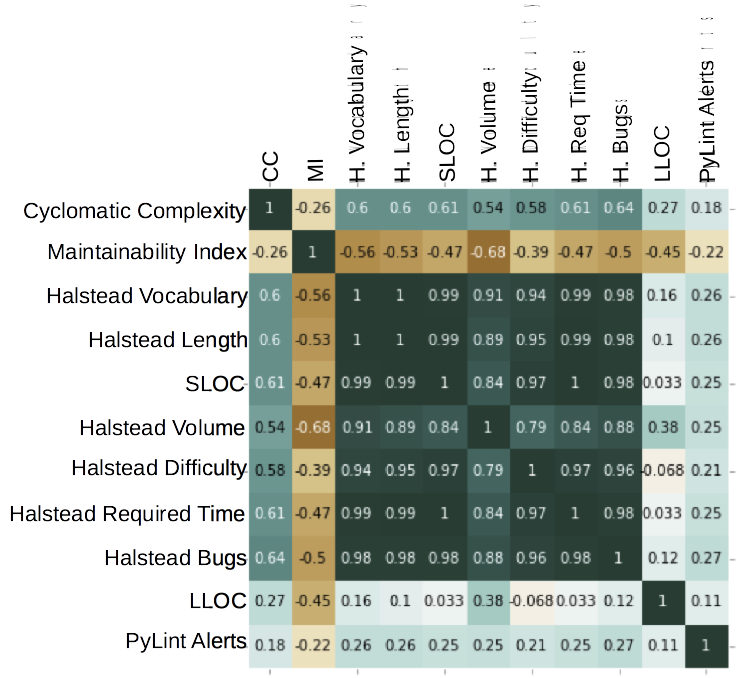
\includegraphics[width=10cm]{images/corr_matrix_11.png}
      \caption{Matriz de correla��o dos 11 atributos extra�dos inicialmente}
      \label{fig:initialcorrelation}
    \end{figure} 

    O teste $\chi^2$ foi aplicado para entender, dentre os atributos relacionados a Halstead, quais s�o os dois mais relevantes. Para este teste, os atributos de Halstead mais relevantes s�o: \emph{Halstead Volume} e \emph{Required Time}. A nova matriz de correla��o calculada (figura~\ref{fig:finalattributes}) demonstra que os 6 atributos selecionados (tabela~\ref{tab:finalattributes}) s�o suficientemente independentes entre si (com exce��o das medidas de Halstead). Observa-se ainda a independ�ncia dos atributos selecionados com o alvo, como ilustrado na figura~\ref{fig:finalattributes}.

    \begin{table}[]
    \centering
    \caption{Lista de atributos selecionados}
    \label{tab:finalattributes}
    \begin{tabular}{@{}|l|c|l|@{}}
    \toprule
    \multicolumn{1}{|c|}{\textbf{\#}} & \textbf{Atributo}                       & \multicolumn{1}{c|}{\textbf{Descri��o}}                            \\ \midrule
    1                                 & Complexidade Ciclom�tica                & N�mero de declara��es                                              \\ \midrule
    2                                 & �ndice de Manutenabilidade              & Corresponde � organiza��o do c�digo                                \\ \midrule
    3                                 & \multicolumn{1}{l|}{Volume de Halstead} & Combina��o entre n�mero de linhas e declara��es                    \\ \midrule
    4                                 & Tempo de Halstead                       & Tempo estimado para compilar um c�digo                             \\ \midrule
    5                                & LLOC                                    & N�mero de linhas l�gicas                                           \\ \midrule
    6                                & Alertas PyLint                          & \begin{tabular}[c]{@{}l@{}}Verdadeiro se PyLint gerou alertas. \\ Caso contr�rio, falso\end{tabular}\\ \bottomrule
    \end{tabular}
    \end{table}

    \begin{figure}[H]
      \centering
      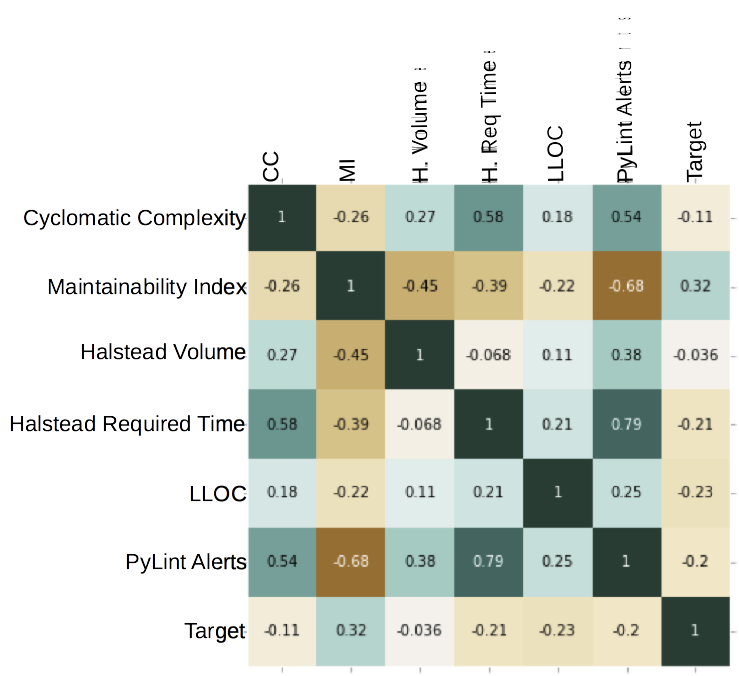
\includegraphics[width=10cm]{images/finalattributes.png}
      \caption{Matriz de correla��o dos 6 atributos selecionados. As correla��es com a sa�da tamb�m s�o calculadas.}
      \label{fig:finalattributes}
    \end{figure} 

    
    \section{Avalia��o dos Classificadores}
    \label{avaliacao} 

Em F�sica de Altas Energias, � comum encontrar a aplica��o de BDT (\emph{Boosted Decision Tree}, ver se��o~\ref{bdt}) para identifica��o de part�culas. No Farmilab, por exemplo, as an�lises para busca de oscila��es de neutrinos deu-se por meio de aplica��o de BDT~\cite{Roe2005577}. No CERN existem diversos trabalhos utilizando BDT para identifica��o do part�culas (~\cite{1748-0221-10-09-P09018}, ~\cite{Chatrchyan2012284} e ~\cite{JenniferGodfrey2009} por exemplo). Portanto, existe um incentivo natural para a aplica��o de m�todos \emph{ensemble} com �rvores neste projeto contextualizado no ambiente do CERN. Como citado, a popularidade de �rvores de decis�o na comunidade cient�fica vem da sua f�cil compreens�o.

    Com os atributos selecionados (se��o~\ref{selection}), classificadores em \emph{ensemble} foram treinados. Para todos os casos, o algoritmo base � uma �rvore de decis�o, gerada previamente. Como sa�das, teremos as classes \emph{execut�vel} indicando que provavelmente o c�digo fonte n�o vai falhar ao ser executado na m�quina \emph{slave} ou, caso contr�rio, \emph{n�o execut�vel}.

    Antes de dividir o conjunto de dados em subconjuntos de treino (70\%) e teste (30\%), foi necess�rio replicar o conjunto com alvo \emph{n�o execut�vel}, devido a despropor��o em n�mero de amostras. � importante ressaltar que os mesmos conjuntos de treino e teste foram utilizados para todos os casos. Como medida de incerteza, foi utilizado o erro quadr�tico m�dio das 100 itera��es realizadas.

    Como avalia��o de performance, foram calculados matrizes de confus�o e F1-scores. Em an�lises estat�sticas de classifica��o bin�ria, o F1-score � uma medida de acur�cia. Ela considera tanto precis�o quanto sensibilidade, como pode ser observado pela f�rmula abaixo:

    \begin{center}
    $F1_{score} = 2 . \frac{p . r}{p + r}$ (V)
    \end{center}
    Na f�rmula (V) $p$ � precis�o e $r$ � sensibilidade (do ingl�s, \emph{recall}).

    Precis�o � o n�mero de verdadeiro positivos dividido pelo n�mero total de resultados positivos. Sensibilidade � o n�mero de verdadeiro positivos dividido pelo n�mero de resultados positivos que deveriam ter sido retornados.

    O F1-score pode ser interpretado como uma m�dia ponderada da precis�o e sensibilidade, onde o melhor valor para avaliar a acur�cia � 1 e o pior, 0.
    \\ \\
    \textbf{\large{�rvore de decis�o}}\\ \\
    O crit�rio \emph{�ndice gini} para divis�o da �rvore de decis�o foi utilizado. Estipulou-se um tamanho m�ximo igual a tr�s, a fim de evitar \emph{overfitting}. Segundo a literatura, � esperado que este classificador tenha um desempenho pior quando comparado com os m�todos em \emph{ensemble}. Esta �rvore foi utilizada como classificador base nos tr�s m�todos descritos a seguir. 
    \\ \\
    \textbf{\large{Bagged Trees}}\\ \\
    Utilizando o mesmo conjunto de treino utilizado para treinar o classificador base e, utilizando a �rvore de decis�o descrita anteriormente, um classificador em \emph{Bagged Tree} foi gerado. No caso, o n�mero de itera��es estabelecido � igual a 100. Ou seja, ao final do treinamento, tem-se 100 �rvores treinadas. O resultado d�-se por voto majorit�rio dessas 100 �rvores. A cada rodada, 10\% do conjunto de treino foi utilizado como sub-conjunto \emph{boostrap} (o equivalente a cerca de 60 amostras). Isso � o suficiente para garantir que as amostras n�o sejam repetidas in�meras vezes, o que mant�m a independ�ncia dos 100 classificadores gerados pelo m�todo.\\ \\
    \textbf{\large{Random Forest}}\\ \\
    Para o classificador em \emph{Random Forest} os mesmos crit�rios estabelecidos para treinar o \emph{Bagged Tree} se aplicam. Mas, o que difere os dois m�todos � a quantidade de atributos utilizados em cada itera��o para treinar uma �rvore. Em~\cite{Breiman:2001:RF:570181.570182}, o Breiman avalia que empiricamente, um n�mero de atributos pr�ximo a $\sqrt{N}$ (sendo N o n�mero total de atributos) � suficiente para obter melhor acur�cia. No caso abordado nesta disserta��o, temos um n�mero de atributos pequeno (e igual a 6), de tal forma que $\sqrt{6} = 2.45$. O n�mero de atributos, ent�o, utilizado para treinar o classificador em \emph{Random Forest} � igual a 3. Como o \emph{OOB error} � calculado a cada itera��o, uma an�lise de relev�ncia de atributos tamb�m pode ser extra�da durante o treinamento deste classificador.\\ \\
    \textbf{\large{Boosted Decision Trees}}\\ \\
    Apesar deste m�todo permitir treinamento por \emph{cross-validation}, o mesmo procedimento utilizado para treinar os classificadores descritos anteriormente foi utilizado (70\% do conjunto para treino e 30\% para teste). O motivo dessa escolha � permitir que a an�lise de performance seja mais justa. Existem diversos algoritmos que determinam como os pesos que ser�o atribu�dos �s amostras erroneamente classificadas em cada itera��o s�o definidos. No caso, o algoritmo \emph{AdaBoost}~\cite{Freund1997} (do ingl�s, \emph{Adaptative Boosting}) foi utilizado. Inicialmente, os pesos atribu�dos equivalem a 1. A cada itera��o o percentual de amostras classificadas de maneira equivocada � calculado e o peso que ser� atribu�do a tais amostras � definido baseado neste percentual. O resultado final depender� tamb�m deste peso calculado a cada itera��o.

    A figura~\ref{fig:adaboost_pseudocode} ilustra um pseudo-c�digo extra�do de~\cite{Freund1997}. Nela � poss�vel entender como o peso $\beta$ � calculado, e tamb�m como o resultado final � obtido.

    \begin{figure}[H]
      \centering
      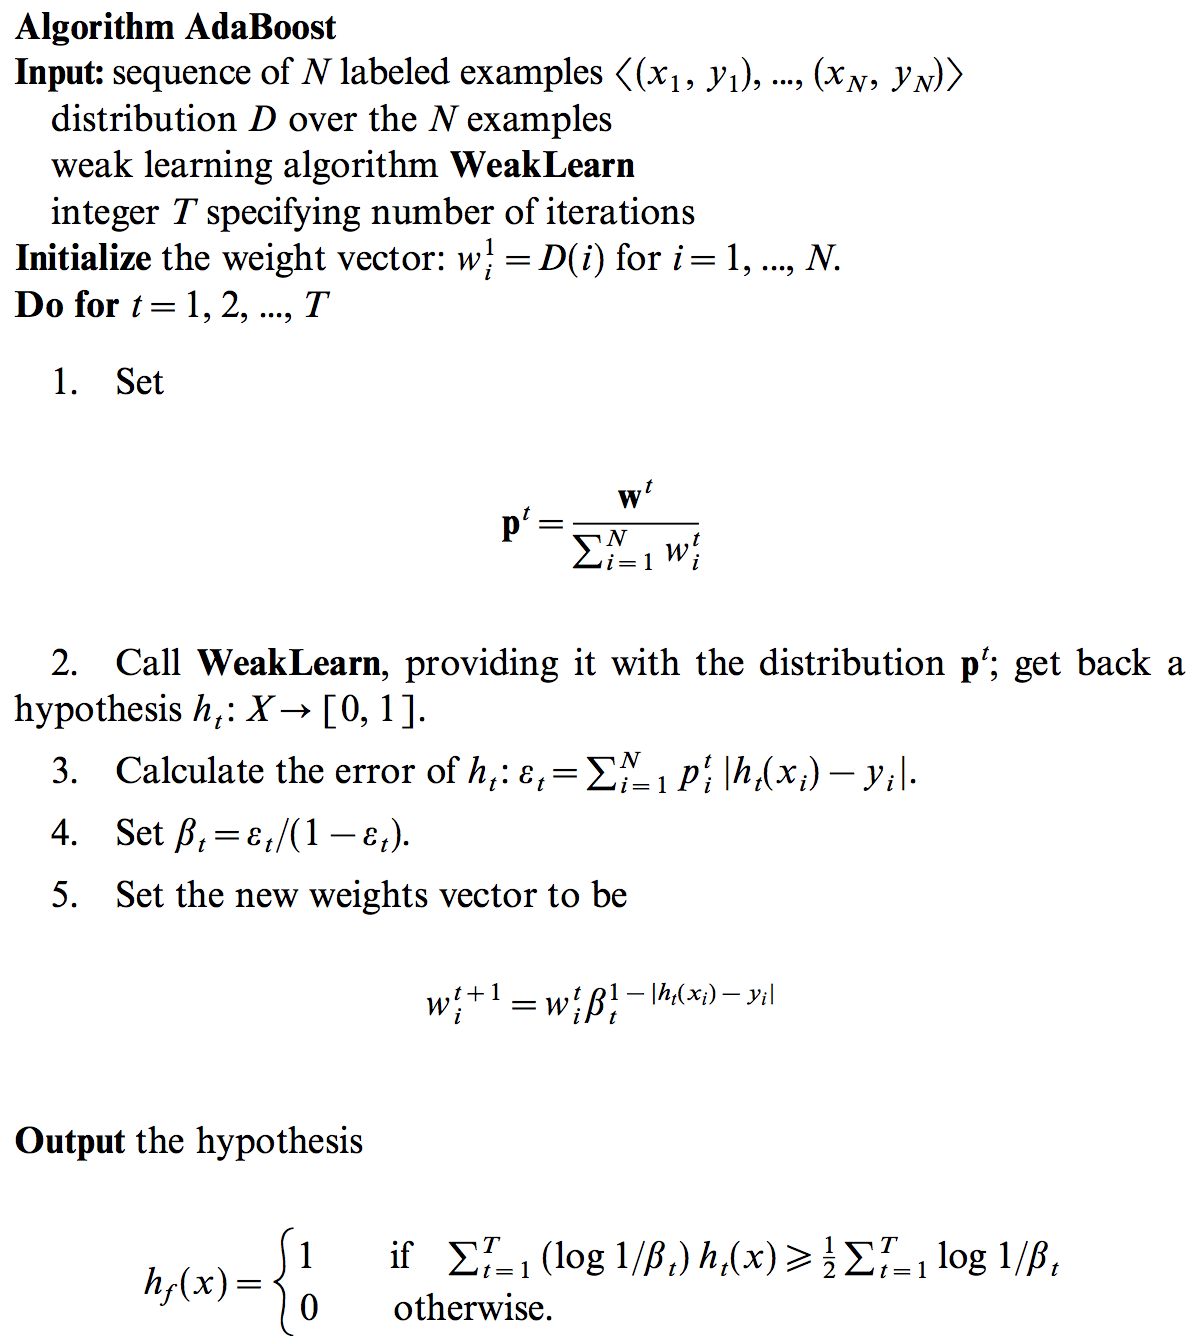
\includegraphics[width=8cm]{images/bdt_pseudocode.png}
      \caption{Pseudo-c�digo do algoritmo \emph{AdaBoost}}
      \label{fig:adaboost_pseudocode}
    \end{figure} 

    As figuras~\ref{fig:confusionmatrices} e~\ref{fig:reports} 
    ilustram as matrizes de confus�o e algumas medidas de desempenho, respectivamente, que foram geradas utilizando o mesmo conjunto de teste para os 4 classificadores gerados.

    No caso da �rvore de decis�o, � esperado que seu desempenho seja pior comparativamente: o tamanho fixado em tr�s e o n�mero m�ximo de folhas fixado em cinco impede que ao final, o classificador gerado possua folhas mais puras. A vantagem dessa abordagem � que desta maneira, � mais dif�cil obter \emph{overfitting}. Por outro lado, uma �rvore de decis�o � insuficiente para se obter generaliza��o.

    Tais quest�es s�o contornadas com a aplica��o dos m�todos \emph{ensemble}, como previsto na teoria. Dos classificadores gerados por tal m�todo, obt�m-se melhor desempenho com o BDT para a classe \emph{n�o execut�vel}. Percebe-se que o n�mero de itera��es estabelecido em 100 j� � suficiente para atingir tal desempenho. Como ilustrado na figura~\ref{fig:reportbdt}, o classificador em BDT apresenta cerca de 90\% para precis�o e sensibilidade nas duas classes (\emph{execut�vel} e \emph{n�o execut�vel}).

    O classificador \emph{Bagged Trees} � capaz de melhorar um pouco a classifica��o quando comparado com a �rvore de decis�o gerada. Isto tamb�m est� coerente com a teoria. Gerar 100 �rvores de decis�o com sub-conjuntos diferentes aumenta a diversidade dos 70\% do conjunto de treino. Tal procedimento � compar�vel ao treinamento por \emph{cross-validation}. Isso explica o melhor desempenho deste classificador quando comparado com a �rvore de decis�o treinada.

    Al�m da varia��o ocorrida no treinamento para gerar o classificador \emph{Bagged Trees}, o \emph{Random Forest} varia tamb�m a quantidade de atributos utilizados no momento do treinamento das 100 �rvores de decis�o em cada itera��o. Esse fato, al�m de melhorar o desempenho da classifica��o, permite que uma avalia��o de atributos mais relevantes seja feita. Em outras palavras, a cada �rvore gerada � poss�vel obter o erro \emph{OOB} e, avalia-lo de acordo com os atributos que participaram daquela itera��o. A figura~\ref{fig:randomforestfeatures} ilustra atrav�s de um gr�fico de barras quais s�o os atributos mais relevantes dos 6 (listados na tabela~\ref{tab:finalattributes}) utilizados para o treinamento da \emph{Random Forest}. � poss�vel perceber que o �ndice de manutenabilidade � o atributo que mais contribui para o treinamento do classificador. A complexidade ciclom�tica chega a ser menos relevante at� que as medidas de Halstead.

    A tabela~\ref{tab:summary} apresenta as medidas de desempenho dos 4 classificadores gerados. Nela � poss�vel identificar o melhor desempenho pelo F1-score do BDT sob os demais classificadores.

    \begin{figure}[!ht]
      \centering
      \mbox{
        \subfigure[�rvore de Decis�o]{
           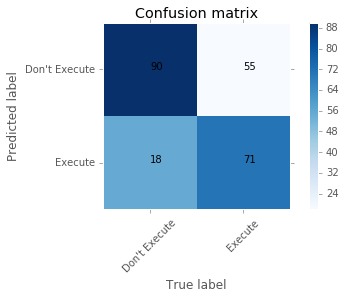
\includegraphics[width=6.5cm]{images/cm_dt.png}
           \label{fig:cmdt}
        }
        \subfigure[Bagged Trees]{
          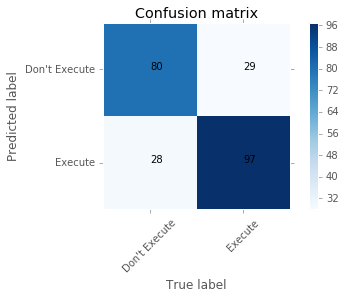
\includegraphics[width=6.5cm]{images/cm_bagged.png}
          \label{fig:cmbagged}
        }
      }
      \mbox{
        \subfigure[Random Forest]{
          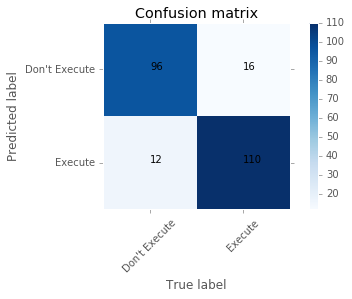
\includegraphics[width=6.5cm]{images/cm_randomforest.png}
          \label{fig:cmrandomforest}
        }
        \subfigure[Boosted Decision Trees]{
           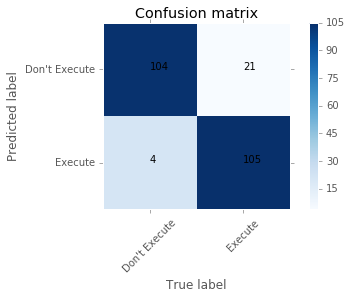
\includegraphics[width=6.5cm]{images/cm_bdt.png}
           \label{fig:cmbdt}
        }
      }
      \caption{Matrizes de Confus�o dos 4 classificadores gerados.}
      \label{fig:confusionmatrices}
    \end{figure}

    \begin{figure}[!ht]
      \centering
        \subfigure[�rvore de Decis�o]{
           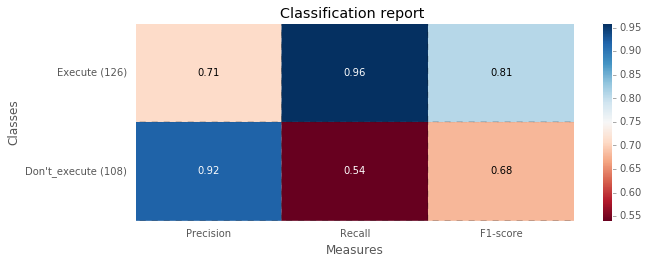
\includegraphics[width=12cm]{images/report_dt.png}
           \label{fig:reportdt}
        }
        \subfigure[Bagged Trees]{
          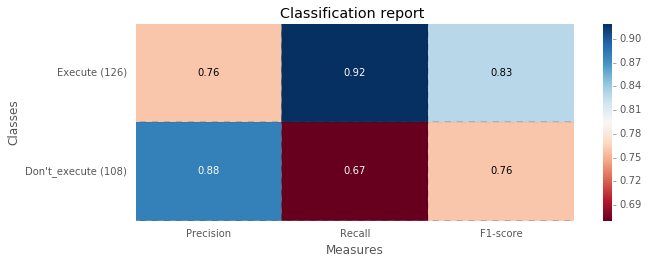
\includegraphics[width=12cm]{images/report_bagged.png}
          \label{fig:reportbagged}
        }
      
        \subfigure[Random Forest]{
          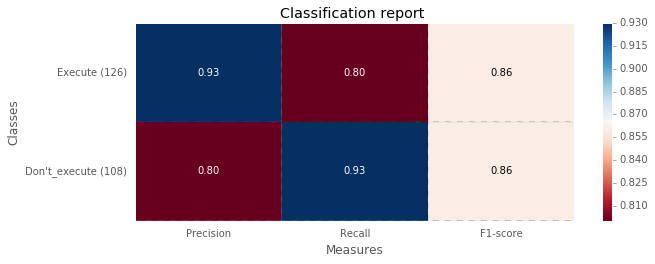
\includegraphics[width=12cm]{images/report_randomforest.png}
          \label{fig:reportrandomforest}
        }
        \subfigure[Boosted Decision Trees]{
           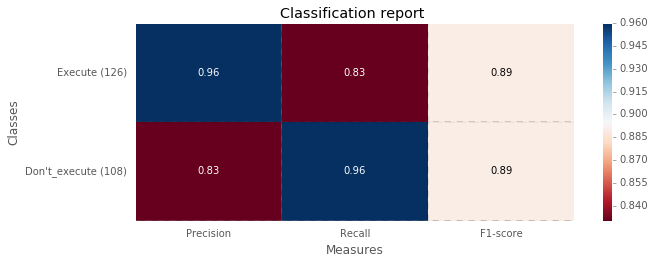
\includegraphics[width=12cm]{images/report_bdt.png}
           \label{fig:reportbdt}
        }
      \caption{Medidas de desempenho dos 4 classificadores gerados.}
      \label{fig:reports}
    \end{figure}

    \begin{figure}[H]
      \centering
      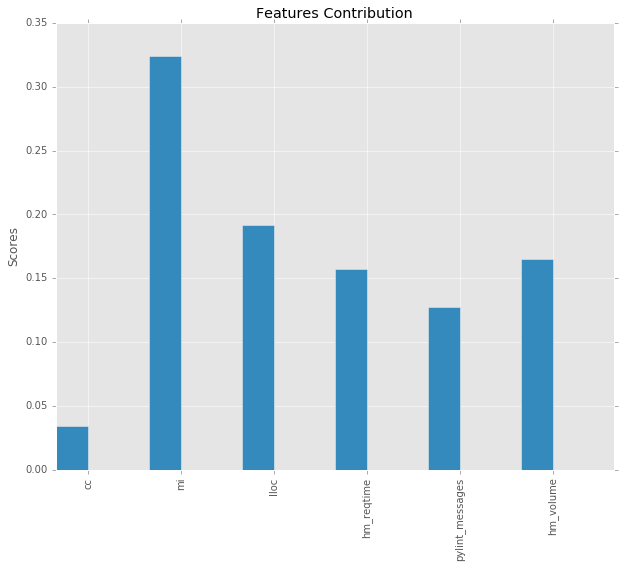
\includegraphics[width=10cm]{images/randomforest_features.png}
      \caption{Atributos mais relevantes de acordo com erro OOB}
      \label{fig:randomforestfeatures}
    \end{figure}

    % Please add the following required packages to your document preamble:
% \usepackage{booktabs}
% \usepackage{multirow}

\begin{landscape}
\begin{table}[]
\centering
\caption{Resumo das medidas de desempenho dos 4 classificadores gerados}
\label{tab:summary}
\begin{tabular}{@{}|c|c|c|c|c|c|c|@{}}
\toprule
\multirow{2}{*}{\textbf{\begin{tabular}[c]{@{}c@{}}Classificador /\\ Classes\end{tabular}}} & \multicolumn{2}{c|}{\textbf{Precis�o (Precision)}}                    & \multicolumn{2}{c|}{\textbf{Sensibilidade (Recall)}}                  & \multicolumn{2}{c|}{\textbf{F1-Score}}                                \\ \cmidrule(l){2-7} 
                                                                                              & \multicolumn{1}{l|}{Execut�vel} & \multicolumn{1}{l|}{N�o execut�vel} & \multicolumn{1}{l|}{Execut�vel} & \multicolumn{1}{l|}{N�o execut�vel} & \multicolumn{1}{l|}{Execut�vel} & \multicolumn{1}{l|}{N�o execut�vel} \\ \midrule
\textbf{�rvore de Decis�o}                                                                    & 0,71 (0,03)                           & 0,92 (0,09)                               & 0,96 (0,04)                            & 0,54 (0,13)                                & 0,81 (0,03)                           & 0,64 (0,11)                                \\ \midrule
\textbf{Bagged Trees}                                                                         & 0,76 (0,02)                           & 0,88 (0,05)                               & 0,92 (0,03)                           & 0,67 (0,12)                               & 0,83 (0,02)                           & 0,76 (0,07)                               \\ \midrule
\textbf{Random Forest}                                                                        & 0,90 (0,01)                            & 0,86 (0,03)                               & 0,87 (0,01)                            & 0,89 (0,01)                               & 0,89 (0,01)                           & 0,87 (0,02)                               \\ \midrule
\textbf{Boosted Decision Trees}                                                                & 0,92 (0,01)                           & 0,89 (0,02)                               & 0,90 (0,03)                           & 0,91 (0,01)                               & \textbf{0,91 (0,02)}                   & \textbf{0,90 (0,01)}                       \\ \bottomrule
\end{tabular}
\end{table}
\end{landscape}
  \chapter{Conclus�es}

  \backmatter
  \bibliographystyle{coppe-unsrt}
  \bibliography{dissertacao}

  \appendix
  \chapter{Alguns casos}
\end{document}